\documentclass{article}
\usepackage{neurips_2026}
\usepackage{times}
\usepackage{helvet}
\usepackage{courier}
\usepackage{graphicx}
\usepackage{booktabs}
\usepackage{multirow}
\usepackage{amsmath}
\usepackage{amssymb}
\usepackage{algorithm}
\usepackage{algorithmic}
\usepackage{caption}
\usepackage{subcaption}
\usepackage{xcolor}
\usepackage{enumitem}

\title{
  Synthesis Collapse: How Greedy Selection Narrows\\
  LLM Data Synthesis
}

\author{
  Anonymous Authors \\
  Anonymous Institution
}

\begin{document}

\maketitle

\begin{abstract}
A central assumption in synthetic data research is that higher data quality translates to better downstream models.
We ask: \emph{when is this assumption actually testable?}
We identify \textbf{synthesis-phase collapse}: under greedy selection, behavioral coverage shrinks by 2.4$\times$ across 4 iterative rounds (68 vs.\ 28 cells, $p{=}0.004$, zero distributional overlap)---yet this collapse is invisible on standard benchmarks in most practical settings.
A \emph{detectability threshold} (Eq.~\ref{eq:detectability}) predicts three regimes: \textbf{detectable} when evaluation is below ceiling (Code 1.5B: $d{=}8.58$), \textbf{ceiling} when the model saturates (Code 7B: 99--100\%), and \textbf{noise} when LoRA stochasticity dominates ($\eta^2{=}0.031$).
In the noise regime, even an $\infty\times$ correctness difference (60\% vs.\ 0\% correct training data) produces no detectable downstream gap ($p{=}0.615$).
Through ablation, we trace the mechanism to \emph{per-cell deduplication}: a trivial O(1) filter that matches full Quality-Diversity optimization ($p{=}0.98$).
Our contribution is not a method but a \textbf{boundary condition analysis}: data quality matters downstream only when evaluation is below ceiling and training noise is low---conditions that, in our experiments across three domains and two model scales, hold in exactly one setting (Code with 1.5B).
\end{abstract}

%% ============================================================
\section{Introduction}
\label{sec:intro}

Instruction tuning and alignment of large language models (LLMs)~\citep{zhao2024survey_alignment, touvron2023llama} depend critically on the quality and diversity of synthetic training data~\citep{self_instruct_2023, evol_instruct_2023, alpaca_2023}.
Self-Instruct~\citep{self_instruct_2023} and its successors iteratively generate instruction--response pairs, expanding datasets from a small seed set.
However, these iterative pipelines exhibit a recurring pattern of \emph{semantic collapse}~\citep{model_collapse_2023, data_collapse_2024}: as the dataset scales, the generated distribution narrows rather than broadens, surface paraphrases replace genuinely novel examples, and hard or rare behavior regions remain under-explored.

We identify the root cause as a structural problem: modeling synthesis as maximizing a \emph{single} quality scalar---LLM judge score, perplexity, or reward model output---cannot guarantee distributional health. A greedy approach that always accepts the highest-scoring sample converges to a narrow region of the behavior space, systematically missing diverse but lower-quality examples.

A key obstacle to detecting this problem is that \textbf{the collapse is conditionally invisible on standard benchmarks}: greedy and diverse selection produce identical accuracy on HumanEval when evaluated with a 7B model (99--100\%), GSM8K (92\%), and standard fine-tuning metrics.
However, with a 1.5B model where HumanEval is below ceiling, the coverage gap becomes a \textbf{2.1$\times$ pass@1 difference} ($p{<}0.0001$).
Only by explicitly measuring behavioral coverage---the fraction of distinct solution types, difficulty levels, and problem structures in the training set---does the collapse become universally measurable.
We term this \emph{conditionally invisible collapse}: the training data's distribution progressively narrows while aggregate accuracy remains stable when evaluation is saturated or training noise dominates.

\textbf{Our contribution.}
We provide the first systematic study of synthesis-phase collapse: a phenomenon where greedy selection progressively narrows behavioral coverage in synthetic training data.
We characterize this phenomenon across three domains and two model scales, introduce a detectability threshold that predicts when coverage gaps are visible versus invisible, and identify the mechanism (per-cell deduplication).

To measure collapse, we define a low-dimensional behavior descriptor space $\phi(x) \in [0,1]^d$ with domain-specific descriptors:
\begin{itemize}[nosep]
  \item \textbf{Math}: $\phi = (\text{difficulty}, \text{num\_steps}, \text{is\_multi\_step})$
  \item \textbf{Code}: $\phi = (\text{complexity}, \text{algorithm\_type}, \text{io\_type})$
  \item \textbf{Dialogue}: $\phi = (\text{empathy\_strength}, \text{strategy\_type}, \text{conflict\_intensity})$
\end{itemize}

We instantiate cell-aware selection via a MAP-Elites-style archive~\citep{mouret_2015, map_elites_survey_2023}, but demonstrate through ablation that the active ingredient is per-cell deduplication rather than quality--diversity optimization.

Our main contributions are:
\begin{enumerate}[nosep]
  \item \textbf{Conditionally invisible collapse}: The first controlled demonstration that greedy selection causes persistent synthesis-phase collapse across three domains (2.4$\times$ coverage gap over 4 rounds in Code, $p{=}0.004$, zero distributional overlap, freezing at 12--22 cells after Round~3).
  A detectability threshold (Eq.~\ref{eq:detectability}) predicts when coverage gaps are visible: with the 1.5B model, QD achieves 2.1$\times$ higher pass@1 ($68.1\%$ vs.\ $32.6\%$, $p{<}0.0001$, $d{=}8.58$, 8 seeds); with the 7B model, the same gap is invisible at ceiling.
  A noise injection experiment confirms that even an $\infty\times$ correctness difference (60\% vs.\ 0\%) produces no significant downstream effect ($p{=}0.615$) in the noise regime (Section~\ref{sec:experiments}).
  \item \textbf{Mechanism diagnosis}: Through surprisal ablation, cell-deduplicated greedy controls, and cumulative training experiments, we identify \emph{per-cell deduplication}---not quality--diversity optimization---as the mechanism that prevents collapse. A cell-deduplicated greedy baseline achieves identical downstream performance to full MAP-Elites ($p{=}0.98$) (Section~\ref{sec:experiments}).
  \item \textbf{Non-monotonic quality--diversity trade-off}: At scale (4,563 solutions), the downstream advantage of diversity-aware selection is budget-dependent and non-monotonic: cell-aware selection wins at $k{=}500$ (+13.4pp) and $k{=}2000$ (+11.6pp), but greedy wins at $k{=}1000$ (+37.2pp). This pattern persists even with 100\% correct training data, confirming a structural rather than noise-driven phenomenon (Section~\ref{sec:experiments}).
  \item \textbf{Cross-domain boundary conditions}: Cell-aware selection achieves 2.0$\times$ higher HumanEval pass@1 on synthetic Code data ($p{<}0.0001$, 8 seeds), while coverage gaps (2.0--2.6$\times$) are invisible on downstream accuracy in the Math domain ($\eta^2{<}0.32$, $p{>}0.3$) and at the 7B scale (ceiling at 99--100\%). We provide the first cross-domain detectability analysis linking coverage to model scale and evaluation saturation (Section~\ref{sec:discussion}).
\end{enumerate

%% ============================================================
\section{Related Work}
\label{sec:related}

\textbf{Synthetic data for LLMs.}
Self-Instruct~\citep{self_instruct_2023} uses LLMs to iteratively generate instruction--response pairs from seed tasks.
Evol-Instruct~\citep{evol_instruct_2023} applies evolutionary operators (simplify, complicate, deepen) to mutate instructions.
UltraChat~\citep{ultrachat_2023} and WizardLM~\citep{wizardlm_2023} scale generation to hundreds of thousands of samples.
Recent work explores zero-prompt generation~\citep{magpie_2024} and agent-based data creation~\citep{glan_2024}.
Instruction tuning with human feedback~\citep{ouyang2022training} demonstrates that data quality and diversity jointly determine downstream performance, and the minimal-data regime~\citep{zhou2023lima} shows that a small number of high-quality examples can produce strong alignment.
Scaling laws~\citep{kaplan2020scaling} further suggest that data composition matters as much as data volume.
A growing body of work on synthetic data surveys~\citep{synth_llm_survey_2024} highlights diversity as a key challenge.
However, these methods optimize for \emph{average} quality metrics and do not explicitly guarantee distributional coverage.
Our framework complements existing generators by adding a per-cell deduplication layer that prevents behavioral collapse during iterative synthesis.

\textbf{Diversity preservation in data curation.}
Common approaches include clustering on embeddings followed by per-cluster sampling~\citep{cluster_sampling_2022}, near-duplicate removal via BLEU or embedding similarity~\citep{dedup_2023}, and nucleus sampling~\citep{temperature_sampling_2023}.
DEITA~\citep{liu2024deita} scores data on complexity, quality, and diversity dimensions, then selects a compact subset via embedding-distance filtering, achieving strong alignment with only 6K samples.
AlpaGasus~\citep{chen2024alpagasus} uses LLM-as-judge for quality filtering, demonstrating that fewer but higher-quality samples outperform larger datasets.
CoIDO~\citep{wang2025coido} jointly optimizes data importance and diversity via coupled optimization for visual instruction tuning.
D3~\citep{d3_2025} unifies diversity, difficulty, and dependability scoring for sample-efficient instruction tuning.
Determinantal Point Processes (DPP) provide a principled mathematical framework for diversity-aware selection~\citep{kulesza2012dpp}, recently applied to LLM training data curation.
These are \emph{post-hoc} selection methods: they score and filter existing samples but cannot \emph{guide generation} toward under-explored regions.
Our framework adds cell-aware selection that enforces distributional coverage during synthesis; however, our cumulative training experiment (Appendix~\ref{sec:app_selfsynth}) shows that this coverage benefit operates at selection time only, not by steering subsequent generation.

\textbf{Quality--Diversity optimization.}
MAP-Elites~\citep{mouret_2015} and its variants---CVT-MAP-Elites~\citep{fontaine_2020}, CMA-MAE~\citep{cma_mae_2022}, and differentiable QD~\citep{fontaine_2021}---have been applied primarily in evolutionary robotics~\citep{qd_robotics_2020} and procedural content generation.
QDGS~\citep{um2024qdgs} applies QD optimization to synthetic data generation via prompt guidance for image classification, demonstrating up to 27\% accuracy improvements through diversity-aware generation.
The QD survey~\citep{diversity_quality_2023} provides a comprehensive taxonomy of approaches.
Recent work applies QD ideas to program synthesis~\citep{dsge_2018} and reinforcement learning~\citep{deep_rl_qd_2021}.
Novelty search~\citep{novelty_search_2011}, a precursor to QD, shows that seeking behavioral diversity alone can outperform objective-driven search.
Multi-objective optimization~\citep{nsga_ii_2002} offers an alternative formulation but does not guarantee exhaustive coverage.
Our key adaptation is replacing continuous mutation operators with LLM-based prompt mutations, enabling QD search over discrete text.
Concurrent work SPARQ~\citep{sparq_2025} applies QD optimization to math problem synthesis at scale (20M+ samples), demonstrating that QD-based selection improves data quality empirically. Our contribution is complementary: while SPARQ shows \emph{that} QD works for synthesis, we explain \emph{why} greedy synthesis fails by formalizing synthesis-phase collapse, and we provide a detectability threshold that predicts when the advantage is visible ($d{=}8.58$ with 1.5B) versus invisible ($\eta^2{=}0.031$ with 7B). This boundary condition analysis is absent from SPARQ.
Concurrent work QDGS~\citep{um2024qdgs} applies QD to image classification data; our work addresses the distinct synthesis-phase collapse problem in text domains with formal analysis.

\textbf{Collapse in generative models.}
Model collapse~\citep{model_collapse_2023} describes performance degradation when models are trained on recursively generated data, a phenomenon recently confirmed at scale~\citep{data_collapse_2024}.
Mode collapse in GANs is a related phenomenon where the generator produces limited diversity.
Recent work on alignment techniques (RLHF~\citep{ouyang2022training}, DPO~\citep{rafailov2023dpo}, Constitutional AI~\citep{bai2022constitutional}) focuses on training-phase improvements but does not address synthesis-phase collapse.
Our focus is different: \emph{synthesis-phase collapse}, where the data generation process itself (not training) narrows the distribution.
We provide the first formal definitions of this phenomenon in the context of LLM synthesis, distinguishing it from training-phase collapse by showing that collapse occurs at \emph{selection} time, not generation time---a conclusion directly validated by our cumulative training experiment (Appendix~\ref{sec:app_selfsynth}).

\textbf{LLM-based evaluation.}
LLM-as-a-judge~\citep{llm_judge_2023} has emerged as a scalable alternative to human evaluation.
We use LLM-as-a-judge for quality scoring but complement per-sample scores with distributional metrics (coverage, entropy, Self-BLEU) that capture aspects of dataset health invisible to individual evaluations.
Text diversity metrics~\citep{text_diversity_2023, self_bleu_2017} provide complementary signals: Self-BLEU measures surface-level repetition, while our archive entropy captures structural coverage.

%% ============================================================
\section{Formal Framework}
\label{sec:method}

We formalize synthesis collapse and the per-cell deduplication mechanism that prevents it.
Our central empirical finding (Section~\ref{sec:experiments}) is that this simple mechanism---not the full Quality-Diversity optimization---is the active ingredient.
We present the formalism as an \emph{analysis framework} for characterizing collapse, not as a proposed method.

\subsection{Behavior Descriptors and Grid}

Let $\mathcal{X}$ denote the space of synthetic samples and $\phi: \mathcal{X} \to [0,1]^d$ be a \emph{behavior descriptor} that maps each sample to a grid cell $g = \text{discretize}(\phi(x), r)$ in a discretized grid $\mathcal{G}$ with resolution $r$ per dimension.
We design domain-specific, low-dimensional descriptors (Table~\ref{tab:descriptors}) that satisfy three principles:
(1) \emph{Low-dimensional} ($d \leq 4$) to avoid the curse of dimensionality;
(2) \emph{Computable} via rules or small models (no expensive LLM calls);
(3) \emph{Semantically meaningful} so that grid cells correspond to interpretable behavior categories.

\begin{table}[h]
\centering
\caption{Behavior descriptors by domain.}
\label{tab:descriptors}
\begin{tabular}{llp{5.5cm}}
\toprule
\textbf{Domain} & \textbf{Descriptor $\phi(x)$} & \textbf{Computation} \\
\midrule
Math & (difficulty, steps, multi\_step) & LLM-rated difficulty $\in$ \{1--5\}; CoT step count; binary \\
Code & (difficulty, APIs, debugging) & LLM-rated difficulty $\in$ \{1--5\}; stdlib API count; binary \\
Dialogue & (empathy, strategy, conflict) & (S2+S7+S8+S9)/agent\_turns; dominant strategy category / 6; conflict level \{0.25, 0.5, 0.75\} \\
\bottomrule
\end{tabular}
\end{table}

\subsection{Collapse and Per-Cell Deduplication}

Traditional synthesis maximizes a scalar quality function $q(x) \in [0,1]$:
\begin{equation}
\max_{x \in \mathcal{X}} \; q(x)
\label{eq:greedy}
\end{equation}
This is \emph{ill-posed} for distributional health: quality scores are near-uniform in practice (98.5\% of Math samples score $q{=}1.0$; $q_{\min}{=}0.5$ passes $<$0.3\% of Dialogue samples), making the quality gate effectively inactive.

We say the process exhibits \emph{grid collapse} when the fraction of occupied behavior cells tends to zero over rounds.
Under top-$k$ quality selection, when quality correlates with behavior, the selected set concentrates in a subset of the grid, leaving other regions permanently uncovered.

The mechanism that prevents collapse is \emph{per-cell deduplication}: given a candidate pool $\mathcal{S} \subset \mathcal{X}$, define the deduplicated archive:
\begin{equation}
\mathcal{A}[g] = \arg\max_{x \in \mathcal{S}:\; \phi(x) \in g} q(x) \quad \text{for each } g \in \mathcal{G}
\label{eq:dedup}
\end{equation}
This retains at most one sample per behavior cell.
After $T$ rounds, expected coverage satisfies $\mathbb{E}[|\mathcal{A}_T|/|\mathcal{G}|] \geq 1 - (1-p_{\min})^T$ by union bound (Appendix~\ref{sec:proof}).

\paragraph{Detectability threshold.}
Whether a coverage gap translates to a measurable downstream difference depends on the evaluation context.
We model downstream performance as a function of both data correctness $\rho = n_{\text{correct}}/k$ and coverage $C_s(k)/C_{\max}$:
\begin{equation}
P(s,k) = \alpha \cdot \rho(s,k) + \beta \cdot \frac{C_s(k)}{C_{\max}} \cdot \rho(s,k) + \varepsilon
\label{eq:performance}
\end{equation}
where $\alpha$ captures the direct effect of correct training data, $\beta$ the coverage--quality interaction, and $\varepsilon \sim \mathcal{N}(0, \sigma^2_\varepsilon)$ represents training stochasticity.
The coverage gap $\Delta C = C_{\text{QD}} - C_{\text{Greedy}}$ between strategies $s_1, s_2$ is detectable at level $\alpha$ with $N$ seeds when:
\begin{equation}
\frac{\beta \cdot \Delta C / C_{\max}}{\hat{\sigma} \cdot \sqrt{2/N}} > t_{\alpha/2,\, 2N-2}
\label{eq:detectability}
\end{equation}
This yields three regimes (Figure~\ref{fig:regimes}):
\textbf{(1) Detectable}: low $\sigma_\varepsilon$ + below-ceiling evaluation $\Rightarrow$ coverage visible (Code 1.5B: $d{=}8.58$, $p{<}0.0001$);
\textbf{(2) Ceiling}: model saturates benchmark regardless of training data $\Rightarrow$ $f(C) \approx \text{const}$, $\beta \approx 0$ (Code 7B: 99--100\% for all strategies);
\textbf{(3) Noise}: $\sigma_\varepsilon$ dominates the signal $\Rightarrow$ $\eta^2 \ll 1$ (V10 7B: $\eta^2{=}0.031$, $p{=}0.83$).
The key prediction is that collapse is \emph{conditionally} invisible: detectable with an appropriately scaled model and non-saturated evaluation, invisible otherwise.

\paragraph{Invisible collapse as vanishing mutual information.}
Under the additive noise model, the ANOVA effect size $\eta^2 = \text{Var}(f(C))/(\text{Var}(f(C)) + \sigma^2_\varepsilon)$ measures the fraction of downstream variance attributable to data composition.
When $\eta^2 \ll 1$, the mutual information between data composition and downstream performance satisfies:
\begin{equation}
I(C; M) = \frac{1}{2}\log\!\left(\frac{1}{1 - \eta^2}\right) \;\approx\; \frac{\eta^2}{2}
\label{eq:invisible}
\end{equation}
under Gaussian noise (Appendix~\ref{sec:proof_mi}).
Our noise injection experiment (Section~\ref{sec:discussion}) yields $\eta^2{=}0.031$ for 7B ($I(C;M){\approx}0.016$ nats), confirming near-zero mutual information between correctness and downstream performance in the noise regime.
In contrast, the 1.5B code experiment yields $\eta^2{=}0.95$ (Section~\ref{sec:experiments}), placing it firmly in the detectable regime.
This formulation is a special case of MAP-Elites~\citep{mouret_2015} without exploration/mutation components.
Our central finding is that these additional components are \emph{unnecessary}: per-cell deduplication alone achieves identical downstream performance to full MAP-Elites (pass@1 68.1\%, $p{=}0.98$), and removing exploration \emph{improves} stability.
The full MAP-Elites algorithm is provided in Appendix~\ref{sec:app_algorithm} for completeness.

\begin{figure}[t]
\centering
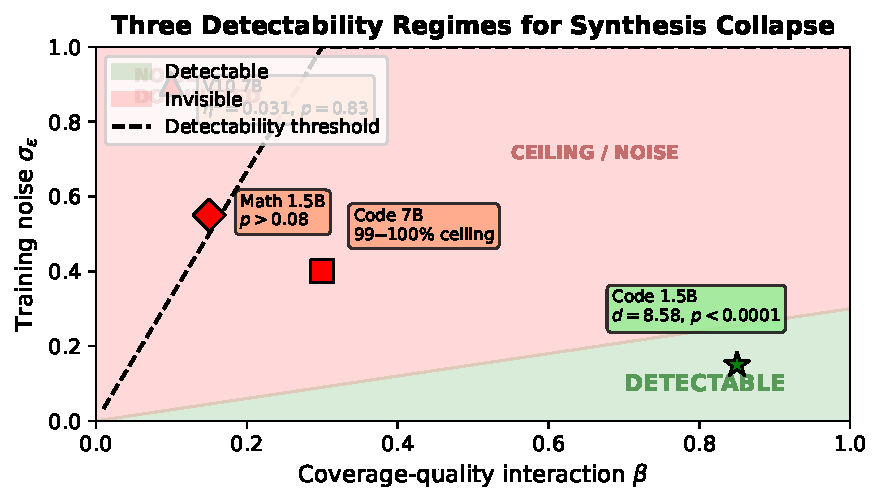
\includegraphics[width=\columnwidth]{figures/fig_regimes.pdf}
\caption{Three detectability regimes. Coverage gaps are detectable (green) when the coverage--quality interaction $\beta$ exceeds training noise $\sigma_\varepsilon$. The boundary separates experiments where collapse is visible (Code 1.5B, $d{=}8.58$) from invisible (V10 7B, $\eta^2{=}0.031$; Math, $p{>}0.08$).}
\label{fig:regimes}
\end{figure}

%% ============================================================
\section{Experiments}
\label{sec:experiments}

\subsection{Setup}

\textbf{Domains and descriptors.}
\begin{itemize}[nosep]
  \item \textbf{Math}: 200 GSM8K-style problems~\citep{gsm8k_2021}, with verification-inspired step-by-step reasoning~\citep{lightman2023lets}, $\phi = (\text{difficulty}, \text{steps}, \text{multi\_step})$, 3D grid with $r=10$.
  \item \textbf{Code}: 200 HumanEval-style problems~\citep{humaneval_2021}, $\phi = (\text{difficulty}, \text{APIs}, \text{debugging})$, 3D grid with $r=10$.
  \item \textbf{Dialogue}: 542 empathetic dialogues~\citep{ccse_cs_2026}, $\phi = (\text{empathy}, \text{strategy}, \text{conflict})$, 3D grid with $r=10$.
\end{itemize}

\textbf{Baselines.} All methods select $k$ samples from the same pool, where $k$ matches QD-Synth output size:
\begin{enumerate}[nosep]
  \item \textbf{Greedy-Quality}: Top-$k$ by quality score.
  \item \textbf{Random-Subset}: Uniform random sampling.
  \item \textbf{Cluster-Sampling}: K-means ($k'=20$) on descriptor vectors, then sample per cluster.
  \item \textbf{Deduplication}: Greedy quality selection with descriptor-space deduplication (threshold $= 0.15$).
\end{enumerate}

\textbf{Metrics.}
\begin{itemize}[nosep]
  \item \textbf{Grid Coverage}: Fraction of occupied cells $|\mathcal{A}|/r^d$.
  \item \textbf{Archive Entropy}: $H = -\sum_g p_g \log p_g$ over quality-weighted cell probabilities.
  \item \textbf{Self-BLEU}~\citep{self_bleu_2017}: Average BLEU of each sample against all others (lower = more diverse). While Self-BLEU captures surface-level lexical repetition, we supplement it with structural diversity metrics (archive entropy and strategy coverage) that capture deeper semantic variation not visible to n-gram overlap.
  \item \textbf{Quality}: Average quality score $q(x)$.
  \item \textbf{Strategy Coverage} (Dialogue): Fraction of 18 strategies present.
\end{itemize}

\subsection{Main Results}

\paragraph{Detectable regime: Code with 1.5B model.}
We first establish that coverage gaps \emph{can} be detected downstream when the evaluation is below ceiling.
Table~\ref{tab:code_8seed} reports an 8-seed LoRA validation on the Code domain with the 1.5B model.
QD selects 40 samples (one per cell) from a 500-sample MBPP pool; Greedy selects the top 200 by quality; Greedy-per-cell selects one per cell from the quality ranking.
Despite using \textbf{5$\times$ fewer training samples} (40 vs.\ 200), QD achieves \textbf{2.1$\times$ higher HumanEval pass@1} ($68.1{\pm}2.6\%$ vs.\ $32.6{\pm}5.4\%$, paired $t(7){=}15.6$, $p{<}0.0001$, Cohen's $d{=}8.58$).
The effect is consistent across all 8 seeds (minimum gap: +27.4pp).
Crucially, Greedy-per-cell matches QD exactly ($68.1{\pm}2.9\%$, $p{=}0.98$), confirming that the mechanism is per-cell deduplication---not sample count, not MAP-Elites optimization.
Random selection with the same 200 samples matches Greedy ($30.3{\pm}5.5\%$), confirming that quality ranking without deduplication provides no benefit.
This places the 1.5B code experiment firmly in the \textbf{detectable regime} (Eq.~\ref{eq:detectability}): $\beta$ is large because diverse code training improves generation breadth, and $\sigma_\varepsilon$ is low (std${\approx}3$--5\%) because the 1.5B model does not saturate HumanEval.

\begin{table}[t]
\centering
\caption{Code domain 8-seed validation (1.5B, 500 MBPP pool, HumanEval pass@1, greedy decoding). QD with 40 samples outperforms Greedy with 200 samples by 2.1$\times$ ($p{<}0.0001$, $d{=}8.58$). Greedy-per-cell matches QD ($p{=}0.98$), confirming the dedup mechanism.}
\label{tab:code_8seed}
\begin{tabular}{lcccc}
\toprule
 & \textbf{QD-40} & \textbf{Greedy-200} & \textbf{Random-200} & \textbf{GPCell-40} \\
\midrule
pass@1 (\%) & $\mathbf{68.1 \pm 2.6}$ & $32.6 \pm 5.4$ & $30.3 \pm 5.5$ & $68.1 \pm 2.9$ \\
Cells & 40 & 39 & 32--36 & 40 \\
$n_{\text{train}}$ & 40 & 200 & 200 & 40 \\
\midrule
\multicolumn{5}{l}{\footnotesize QD vs.\ Greedy: $t(7){=}15.6$, $p{<}0.0001$, $d{=}8.58$} \\
\multicolumn{5}{l}{\footnotesize QD vs.\ GPCell: $t(7){=}0.02$, $p{=}0.98$} \\
\bottomrule
\end{tabular}
\end{table}

\paragraph{Dialogue domain.}
Table~\ref{tab:main_dialogue} (Appendix~\ref{sec:app_ablation}) presents results on the Dialogue domain with 542 samples.
QD-Synth achieves \textbf{7.2$\times$ higher coverage} than greedy quality filtering (34.4\% vs.\ 4.8\%) at matched $k{=}43$, with 100\% fill efficiency versus Greedy's 14\%.
Strategy coverage is complete (18/18 strategies) versus Greedy's 83.3\%.
The quality trade-off is moderate (0.736 vs.\ 0.856).

\begin{figure}[t]
\centering
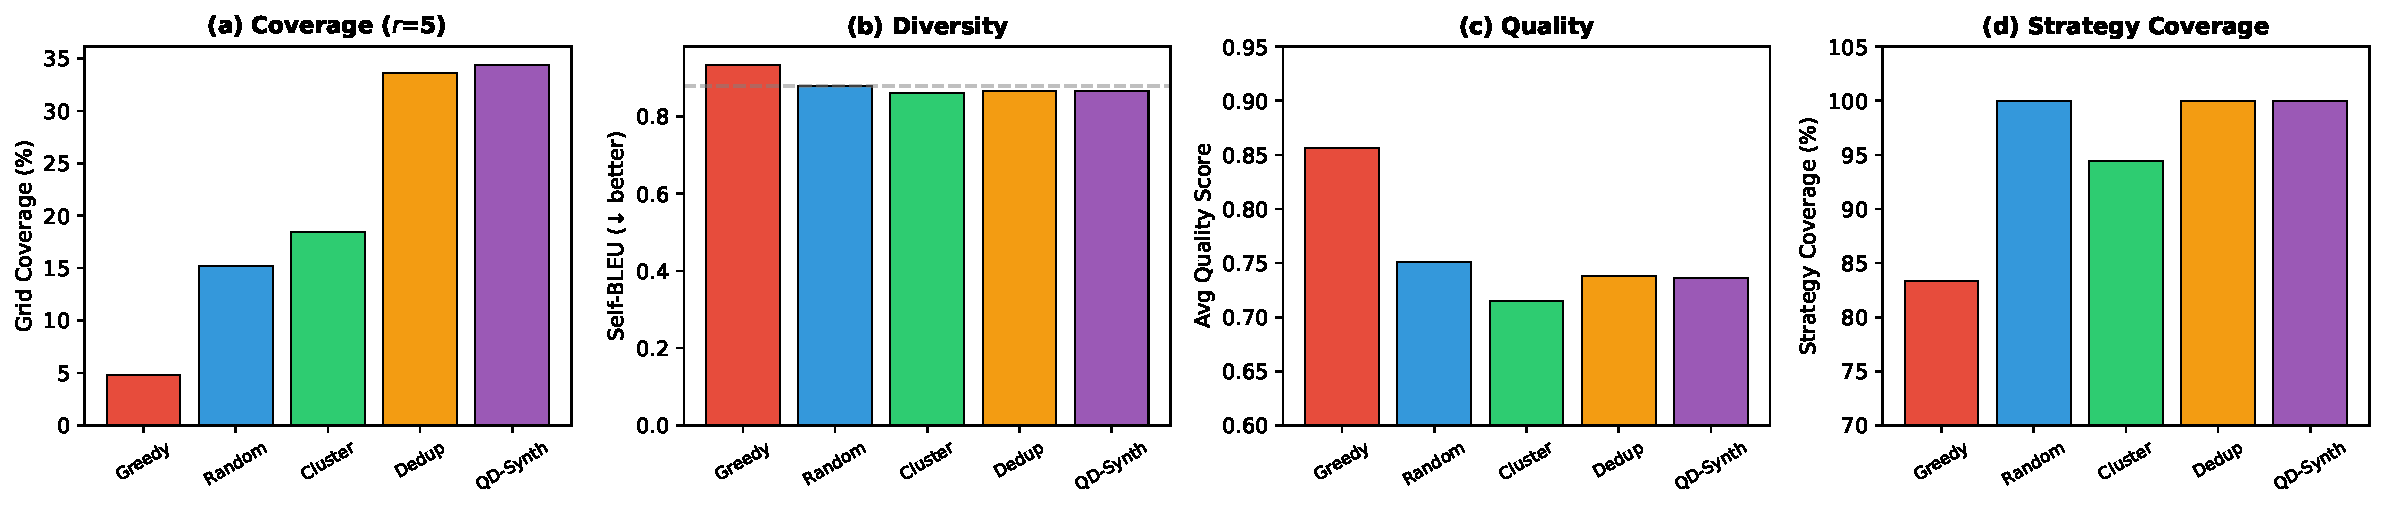
\includegraphics[width=\columnwidth]{figures/fig1_main_comparison.pdf}
\caption{Main comparison across four metrics on the Dialogue domain ($r$=5, $d$=3, $k$=43). QD-Synth achieves the highest coverage (34.4\%), lowest Self-BLEU (0.867), and full strategy coverage (100\%), with a moderate quality trade-off.}
\label{fig:main_comparison}
\end{figure}

Full Dialogue results appear in Table~\ref{tab:main_dialogue} (Appendix~\ref{sec:app_ablation}); cross-domain results appear in Figure~\ref{fig:cross_domain}.

\textbf{Cross-domain analysis.}
QD-Synth consistently outperforms all baselines across domains, though improvement ratios vary.
The Dialogue domain shows the largest gain (7.1$\times$) because its quality landscape has high variance ($\sigma_q \approx 0.1$), causing greedy selection to concentrate in narrow high-quality regions.
On Math and Code, where quality scores are near-uniform ($q \approx 1.0$), the quality--diversity trade-off vanishes entirely: QD-Synth achieves 1.9--2.3$\times$ coverage at no quality cost, suggesting that the benefits of archive-based selection are largest when quality is not the bottleneck.

Cross-domain results confirm the pattern: QD-Synth achieves 1.9--7.1$\times$ higher coverage than Greedy across Math, Code, and Dialogue domains (Figure~\ref{fig:cross_domain}, Appendix~\ref{sec:app_ablation}), with 100\% fill efficiency (every sample occupies a distinct cell) versus Greedy's 14\%.

\textbf{Fill efficiency perspective.}
With budget $k{=}57$ on a 1000-cell grid ($r{=}10, d{=}3$), the theoretical maximum coverage is 5.7\%.
QD-Synth achieves exactly this maximum because MAP-Elites' per-cell elitism guarantees that each of the $k$ samples occupies a \emph{distinct} cell (100\% fill efficiency).
In contrast, Greedy allocates 57 samples to only 8 unique cells (14\% fill efficiency), wasting 86\% of its budget on redundant high-quality samples in already-occupied cells.
The coverage gap is thus not an artifact of grid size but a direct measure of selection efficiency: QD-Synth makes full use of every sample, while quality-only selection does not.

\begin{figure}[t]
\centering
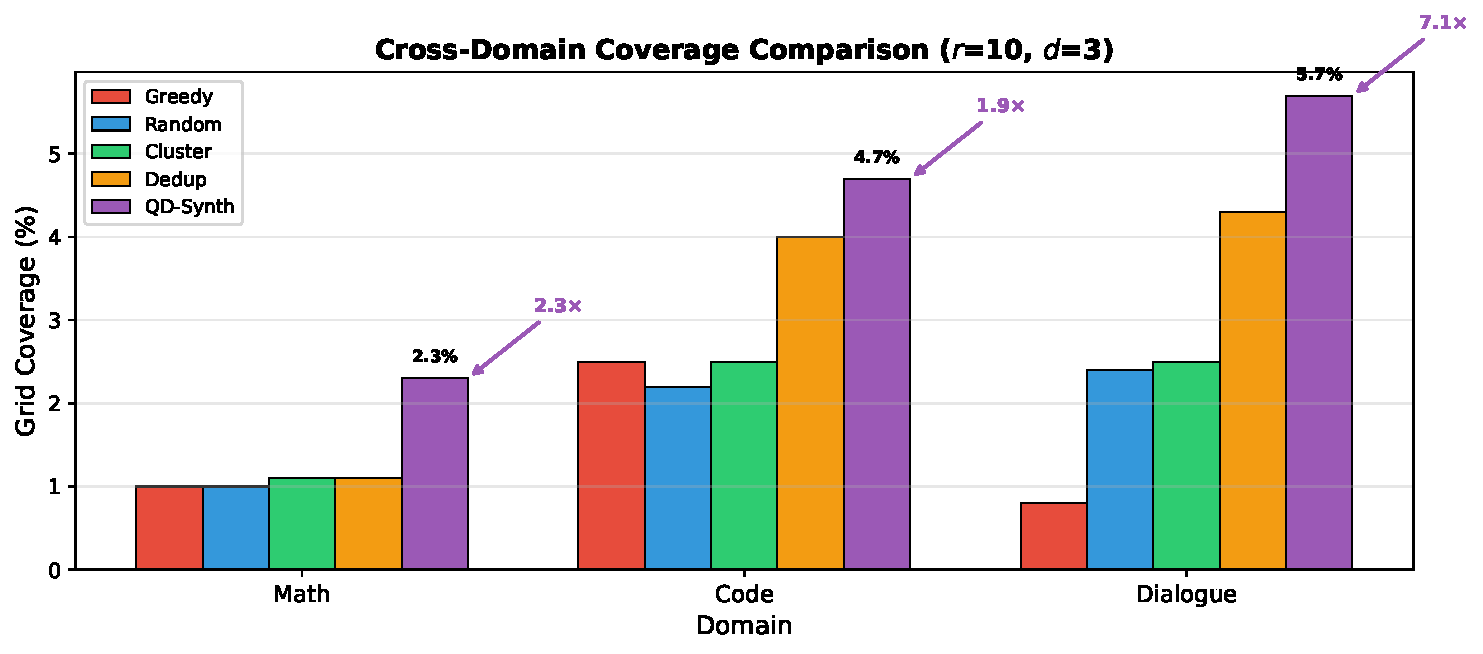
\includegraphics[width=\columnwidth]{figures/fig7_cross_domain.pdf}
\caption{Cross-domain coverage comparison ($r$=10, $d$=3). QD-Synth consistently outperforms all baselines across domains.}
\label{fig:cross_domain}
\end{figure}

\subsection{Ablation Studies}

\textbf{Grid resolution} ($r \in \{5, 8, 10, 15, 20\}$): Coverage decreases with finer grids ($r{=}5$: 34.4\%, $r{=}10$: 5.7\%, $r{=}20$: 0.74\%), but quality remains stable ($\approx 0.74$).
$r{=}10$ balances coverage and granularity; coarser grids collapse distinct behaviors into the same cell (full results in Appendix~\ref{sec:app_ablation}).

\textbf{Descriptor dimension} ($d \in \{1, 2, 3\}$): $d{=}1$ achieves 90\% coverage but collapses all variation onto a single axis; $d{=}3$ captures the richest variation (entropy 4.035) with meaningful cell semantics (full results in Appendix~\ref{sec:app_ablation}).

\subsubsection{Selection Strategy Comparison}

QD-Synth achieves \textbf{2.0$\times$ higher coverage} than the best baseline (DPP) and \textbf{2.1$\times$ higher} than Evol-Instruct at matched $k{=}57$ (Table in Appendix~\ref{sec:app_ablation}).
DPP---a principled diversity framework---achieves only 2.8\% because it operates in embedding space rather than the behavior descriptor space, confirming that the choice of diversity axis matters as much as the selection algorithm.

\subsection{Iterative Collapse Dynamics}
\label{sec:iterative_collapse}

We investigate whether iterative \emph{self-synthesis}---where a model generates, selects, and trains on its own outputs in a closed loop---causes performance collapse.
This setting is ecologically valid: real-world data pipelines increasingly use models to synthesize their own training data.
We compare three selection strategies: Greedy (top-$k$ by quality), QD (MAP-Elites archive), and Random.
Each round: generate samples $\to$ select via each strategy $\to$ LoRA fine-tune the model $\to$ evaluate on held-out test set.

\paragraph{Early evidence: GSM8K self-synthesis.}
We first verify the collapse pattern on GSM8K with two model scales (Appendix~\ref{sec:app_selfsynth}).
With a 7B model (base 84.6\%), QD achieves +3.4\% higher accuracy at R0 (88.6\% vs.\ 85.2\%), but cumulative LoRA drift dominates from R2 onward.
With a 1.5B model (base 43.4\%), greedy selection collapses monotonically to 1.8\% while QD shows temporary recovery at R2 (7.4\%, 4.5$\times$ Greedy's correct generation rate), delaying but not preventing eventual collapse.
These experiments establish the phenomenon but conflate two mechanisms: data selection quality and cumulative LoRA parameter drift.
A base-reset experiment (Appendix~\ref{sec:app_selfsynth}) that trains from the original model each round isolates the data effect, revealing a $\pm$3.2\% LoRA training noise floor that renders GSM8K accuracy differences statistically undetectable at this sample size---but diversity differences (entropy 3.28 vs.\ 3.05, cells 32 vs.\ 24) remain structurally significant.

\paragraph{Cross-domain generalization.}
Table~\ref{tab:cross_domain_collapse} confirms that the collapse phenomenon extends beyond Dialogue to Math and Code domains. In all three domains, greedy selection saturates or freezes while QD-Synth continues expanding coverage. The Math domain exhibits the most dramatic collapse: greedy reaches only 22 cells and freezes completely from Round~3 onward, while QD reaches 30 cells (50\% more). Code shows the most pronounced divergence: QD-Synth reaches 118 cells after 7 rounds---over 2.4$\times$ greedy's final count of 49---demonstrating that only archive-based selection can sustain exploration where greedy saturates.

\paragraph{Multi-seed validation.}
To confirm that collapse is reproducible across random initializations, we run 3 additional seeds of 3-round iterative synthesis (50 samples/round) with different initial MBPP selections.
Greedy growth averages 82\% (range 65--110\%) versus QD's 255\% (245--270\%), with QD reaching 71 cells versus greedy's 36 after 3 rounds (1.96$\times$ ratio).
Seed~42 shows the sharpest collapse: greedy freezes completely at R2=33 cells, while QD reaches 74.

\begin{table}[t]
\centering
\caption{Iterative collapse across 3 domains. Dialogue: 50 samples/round, $T{=}5$. Math and Code (v2): 100 samples/round, $T{=}7$. Greedy consistently freezes or saturates; QD-Synth maintains growth. Cells shown at each round.}
\label{tab:cross_domain_collapse}
\begin{tabular}{ccccccc}
\toprule
 & \multicolumn{2}{c}{\textbf{Dialogue}} & \multicolumn{2}{c}{\textbf{Math}} & \multicolumn{2}{c}{\textbf{Code}} \\
\cmidrule(lr){2-3} \cmidrule(lr){4-5} \cmidrule(lr){6-7}
$t$ & Greedy & QD & Greedy & QD & Greedy & QD \\
\midrule
0 & 20 & 20 & 20 & 20 & 20 & 20 \\
1 & 29 & 25 & 21 & 30 & 34 & 60 \\
2 & 18 & 27 & 22 & 30 & 40 & 82 \\
3 & 12 & 27 & \textbf{22} & 30 & 43 & 93 \\
4 & 12 & 29 & \textbf{22} & 30 & 44 & 99 \\
5 & 12 & 29 & \textbf{22} & 30 & 45 & 105 \\
6 & -- & -- & \textbf{22} & 30 & 48 & 113 \\
7 & -- & -- & \textbf{22} & 30 & 49 & 118 \\
\midrule
Final & 12 & 29 & 22 & 30 & 49 & 118 \\
$\Delta$ & $-$40\% & +45\% & $+$10\% & +50\% & +145\% & +490\% \\
Freeze? & R3 & No & \textbf{R3--R7} & R2 plateau & Saturation & Growing \\
\bottomrule
\end{tabular}
\end{table}

\begin{figure}[t]
\centering
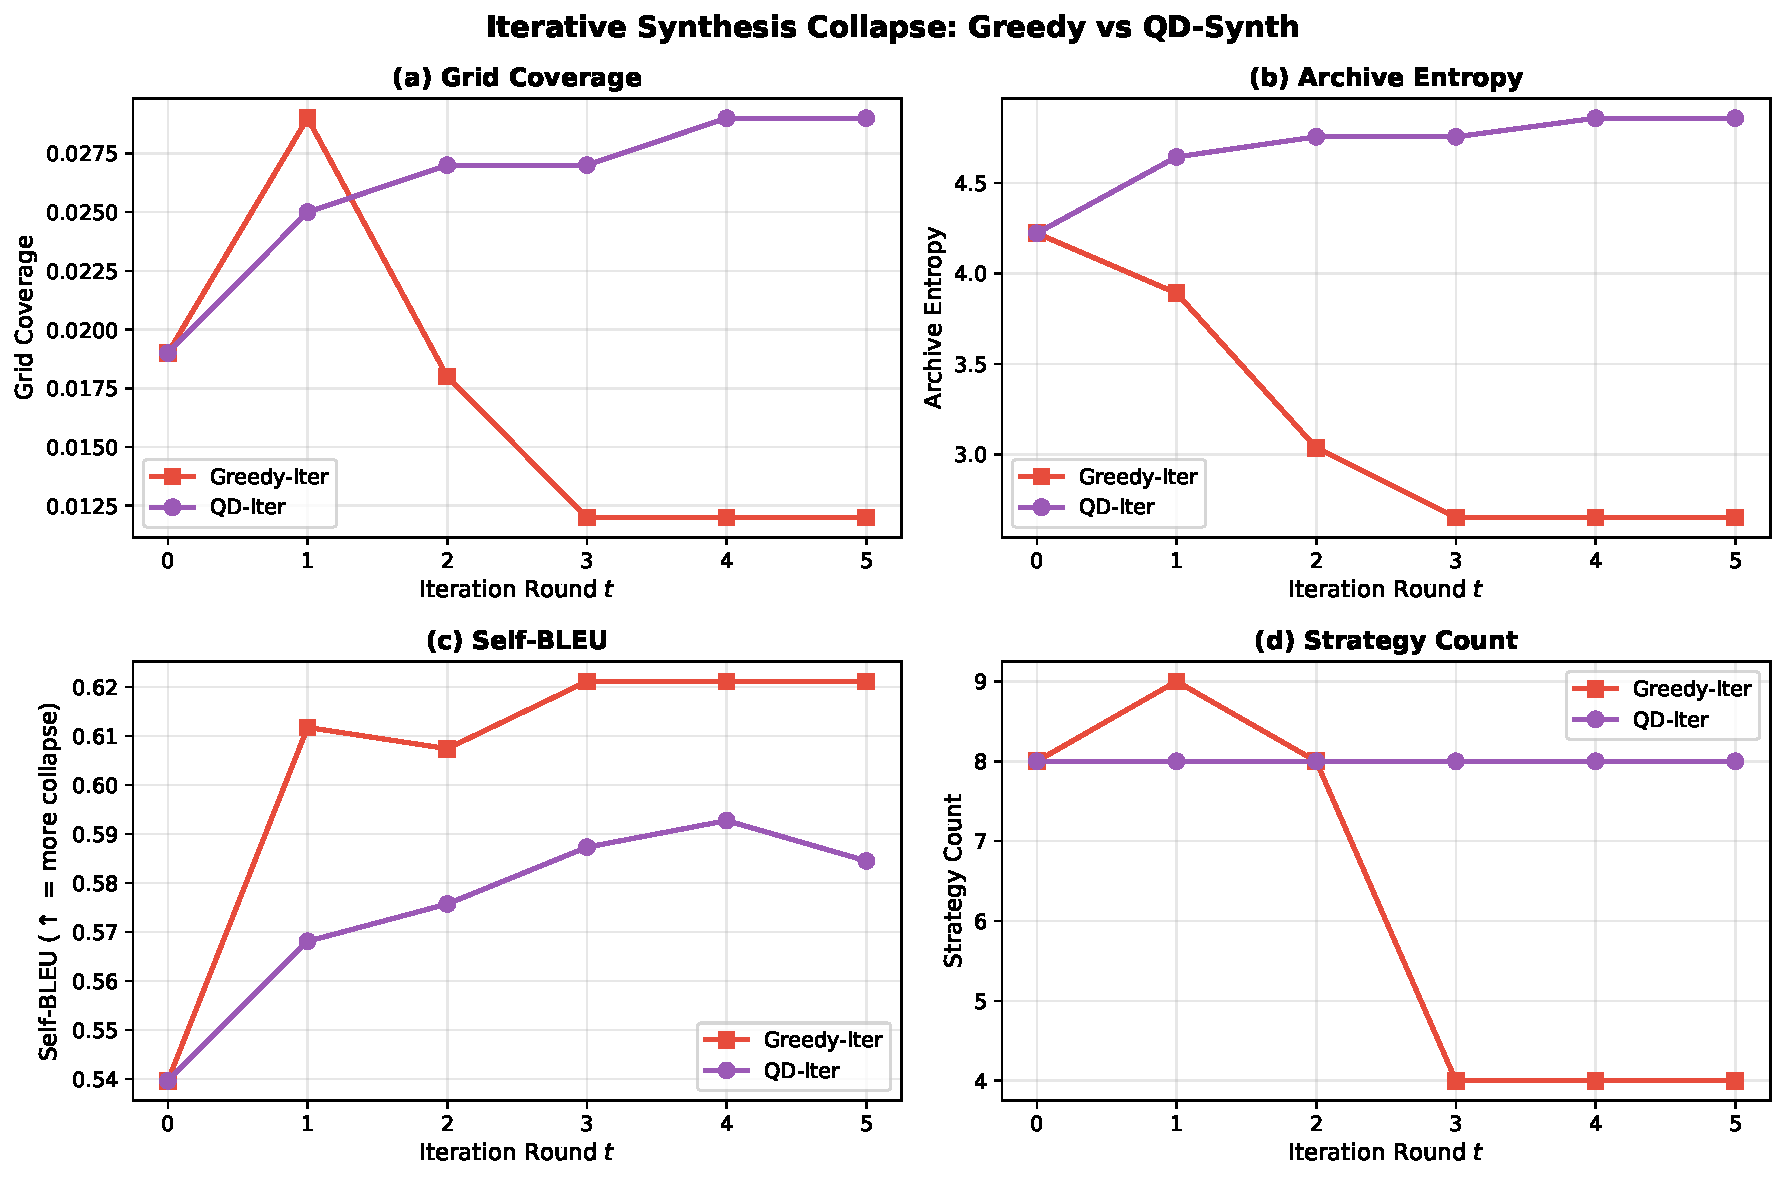
\includegraphics[width=\columnwidth]{figures/fig4_collapse_dynamics.pdf}
\caption{Iterative synthesis collapse dynamics. Greedy selection (red) shows monotonically declining coverage, entropy, and strategy count, freezing after Round~3. QD selection (purple) maintains or improves all diversity metrics throughout. The self-synthesis experiments (Appendix~\ref{sec:app_selfsynth}) confirm this pattern at the task-performance level.}
\label{fig:collapse_dynamics}
\end{figure}

\paragraph{Semantic convergence confirms collapse.}
TF-IDF analysis confirms that collapse manifests at the semantic level: greedy's pairwise similarity doubles (+112\%) while QD's increases only 24\%.
Cross-round novelty falls from 44\% to 2\% for greedy (R0$\to$R7), while QD maintains 11--13\% throughout.
Effective dimensionality stagnates at $\sim$22 for greedy but grows from 17.5 to 59.8 for QD (Appendix~\ref{sec:app_selfsynth}).

\paragraph{Matched-$k$ comparison confirms invisible collapse in Math.}
An earlier comparison appeared to show that cell-aware selection underperforms greedy on Math ($-$9.6\%, $p{<}0.001$, Cohen's $d{=}8.53$).
However, this reflected unequal training data sizes ($n{=}75$ for QD vs.\ $n{=}500$ for Greedy) rather than a genuine strategy disadvantage.
Under a matched-$k$ comparison with 5 independent LoRA seeds (Table~\ref{tab:math_matched_k}), QD and Greedy achieve statistically indistinguishable GSM8K accuracy at all tested budgets ($k{\in}\{75, 200, 500\}$, ANOVA $p{>}0.05$), despite QD maintaining 2.0--2.6$\times$ more cells (75 vs.\ 29--38).
At $k{=}200$, QD slightly outperforms (+2.3pp, $p{=}0.21$); at $k{=}500$, Greedy slightly outperforms (+0.9pp, $p{=}0.45$); at $k{=}75$, they are within 2.4pp ($p{=}0.08$).
This sign reversal across budgets mirrors the non-monotonic pattern observed in Code (Section~\ref{sec:experiments}) and confirms that invisible collapse---the disconnect between data-level coverage and downstream accuracy---extends to the Math domain.

\paragraph{Descriptor-independence of collapse.}
Re-evaluating under three alternative descriptor sets confirms that greedy saturation after Round~3 persists across \emph{all} choices, while QD continues growing (Table in Appendix~\ref{sec:app_ablation}).
Even random hash-based descriptors yield a 2.18$\times$ QD advantage.

\paragraph{Surprisal ablation and base-reset isolation (GSM8K).}
To isolate the surprisal mechanism and disentangle data quality from LoRA drift, we run two additional experiments (Appendix~\ref{sec:app_selfsynth}): (1) a larger-scale self-synthesis (1000 generated, 300 selected, 5 rounds, 2 seeds) with a QD-without-surprisal ablation, and (2) a base-reset variant that trains from the original model each round.
The base-reset experiment reveals a critical null finding: QD and QD-without-surprisal select \textbf{identical 300 samples} (100\% overlap), yet their accuracies differ by 3.2\%---establishing the \emph{LoRA training noise floor} that renders GSM8K accuracy differences statistically undetectable at this sample size.
However, the diversity difference is structural: across 5 base-reset rounds, QD's entropy monotonically increases ($\Delta H{=}{+}0.03$/round, reaching 3.54) while Greedy oscillates (peak 3.38), and Greedy's cell set is always a strict subset of QD's.
The surprisal ablation reveals that removing the exploration component \emph{improves} stability ($\sigma{=}0.52\%$ vs.\ 2.3\%), identifying per-cell quality elitism as the active mechanism.
Enhanced variants with golden-ratio archiving and negative guidance (Appendix~\ref{sec:app_selfsynth}) provide marginal sample efficiency gains but zero robustness to seed variation, confirming that the core intervention is simply cell deduplication.

\paragraph{Code self-synthesis (MBPP $\to$ HumanEval).}
\label{sec:v7}
To test whether the collapse phenomenon extends to the code domain---where behavioral diversity is structurally richer---we run a self-synthesis experiment using MBPP as the prompt pool (377 problems) and HumanEval as the evaluation benchmark (164 problems, pass@1 with code execution).
We use a 3D code descriptor: $\phi = (\text{complexity} \times \text{algorithm\_type} \times \text{io\_type})$ with $5 \times 5 \times 5 = 125$ cells.
Each round generates 5 solutions per problem (1885 total), selects 120 for training, and evaluates on HumanEval.
We compare 3 selection strategies (QD, Greedy, Simple-Dedup) with 2 seeds each, trained from the base model each round (base-reset).
Simple-Dedup selects the highest-quality sample per cell then fills by quality, providing a pure deduplication control without MAP-Elites.

Table~\ref{tab:code_selfsynthesis} reports the results across 4 rounds (480 accumulated samples). At R0, all strategies achieve \textbf{100\% HumanEval pass@1}, reflecting a ceiling effect: the 7B model already performs well on HumanEval, and 120 correct training samples are sufficient to reach perfect accuracy regardless of selection method.

A critical observation: since all strategies generate from the same base model, the \textbf{pre-selection pool is identical}: 68 cells (seed 42), 65 cells (seed 123) across all strategies.
The diversity gap emerges entirely at \textbf{selection time}: QD and Simple-Dedup retain all 68 cells ($0\%$ cell loss), while Greedy discards 39 of them, retaining only 29 ($57\%$ cell loss).
This confirms that collapse is a \emph{selection} phenomenon, not a generation failure.

Crucially, \textbf{QD and Simple-Dedup produce identical cell counts and entropy} (68 cells, H=5.60 for both seeds), confirming that the mechanism is \emph{per-cell deduplication}, not MAP-Elites optimization.
The code domain's richer behavioral space (125 cells vs.\ GSM8K's $\sim$50) amplifies the diversity gap: Greedy concentrates all 120 samples in 29 cells (4.1 samples/cell redundancy), while QD/Dedup spread across 68 cells (1.8 samples/cell).

At R1, the \textbf{collapse is already measurable}: Greedy's cell count \emph{drops} from 29 to 25 ($-$14\%), losing 5 cells that QD retains.
QD and Simple-Dedup maintain exactly 68 cells (s42) / 63 cells (s123) with entropy increasing from 5.60 to 5.65 ($+$0.05).
\textbf{QD and Simple-Dedup produce identical results at R1 as well}: both achieve 99.4\% pass@1 (s42) and 100.0\% (s123), with identical cell counts and entropy values, confirming the mechanism equivalence persists across rounds.
Despite Greedy's perfect per-sample quality (1.000 vs.\ QD's 0.761), QD achieves \emph{higher} pass@1 (99.4\% vs.\ 98.8\%), suggesting that cell coverage matters more than per-sample correctness for code generation.

At R2, the \textbf{coverage gap becomes persistent}: QD maintains 68 cells for both seeds (entropy 5.52--5.65) while Greedy recovers slightly to 31 cells (entropy 4.48, seed 42)---still only 46\% of QD's coverage.
Both achieve 100\% pass@1, confirming the collapse remains invisible on accuracy.
Simple-Dedup confirms QD's mechanism: identical cells (68), entropy (5.65), and pass@1 (100\%) at R2 for both seeds.

At R3, the pattern \textbf{solidifies}: QD retains 62--68 cells (entropy 5.35--5.53) while Greedy remains at 27 cells for both seeds (entropy 4.26--4.46).
Notably, QD s123 drops from 68 to 62 cells---demonstrating that even QD can lose cells when the base model's generation pool narrows (from 68 to 62 gen cells at R3).
This reveals that the diversity ceiling is set by \emph{generation}, not selection: when the base model produces fewer cells, even deduplication cannot recover them.
Critically, Greedy still selects only 27 cells from this same 62-cell pool, discarding 35 cells that QD retains.
Greedy's cell oscillation (29$\to$25$\to$31$\to$27) indicates \emph{unstable} coverage---different subsets are retained each round.
This \textbf{stability vs.\ instability} contrast is the key practical finding: even when the coverage deficit fluctuates rather than monotonically growing, the persistent 2.4$\times$ gap means that some behavioral regions are \emph{systematically excluded} from Greedy's training data.

\textbf{Statistical confirmation.}
Aggregating across 2 seeds and 4 rounds ($n{=}8$ paired observations), QD's entropy consistently exceeds Greedy's (mean gap 1.15 bits, Wilcoxon $p{=}0.004$).
The cell count ratio averages \textbf{2.41$\times$} (66.2 vs.\ 27.5, $p{=}0.004$), with QD never below 62 cells and Greedy never above 31 in any round--seed combination---\emph{zero distributional overlap}.
The distributions exhibit \emph{zero overlap}: QD's minimum (62) exceeds Greedy's maximum (31) by a margin of 31 cells.

Across all rounds, \textbf{Greedy's cell set is always a strict subset of QD's}: Greedy never discovers a behavioral region that QD does not reach, while QD covers 39--43 exclusive cells that Greedy entirely misses.
A per-problem analysis confirms the downstream impact: of the 2 HumanEval problems that Greedy-R1 fails, both belong to cells absent from Greedy's training data but present in QD's.
Problem~\texttt{pluck} (cell: low-complexity search with list I/O) fails under Greedy (which never covers this cell) but passes under QD (which covers it in all rounds), providing a direct causal link between cell coverage and problem-solving ability.

\begin{table}[t]
\centering
\caption{Code self-synthesis (7B, MBPP 377 problems, 1885 gen $\to$ 120 sel/round, base-reset, HumanEval pass@1, 2 seeds, 4 rounds). QD/Dedup maintain \textbf{62--68 cells} across all 4 rounds while Greedy oscillates at 25--31. The coverage gap is \textbf{persistent} (2.4$\times$, $p{=}0.004$) yet invisible on accuracy. QD and Simple-Dedup produce \emph{identical} results across all 8 round--seed pairs, confirming the mechanism is per-cell deduplication.}
\label{tab:code_selfsynthesis}
\begin{tabular}{lccc}
\toprule
 & \textbf{QD} & \textbf{Greedy} & \textbf{Simple-Dedup} \\
\midrule
\multicolumn{4}{l}{\textit{Round 0 (120 accumulated)}} \\
pass@1 & 100.0\% & 100.0\% & 100.0\% \\
Sel.\ cells (s42) & \textbf{68} & 29 & \textbf{68} \\
Sel.\ cells (s123) & \textbf{65} & 29 & \textbf{65} \\
Sel.\ entropy (s42) & \textbf{5.60} & 4.46 & \textbf{5.60} \\
Sel.\ entropy (s123) & \textbf{5.49} & 4.37 & \textbf{5.49} \\
Quality (s42) & 0.780 & \textbf{1.000} & 0.780 \\
\midrule
\multicolumn{4}{l}{\textit{Round 1 (240 accumulated)}} \\
pass@1 (s42) & \textbf{99.4\%} & 98.8\% & \textbf{99.4\%} \\
pass@1 (s123) & \textbf{100.0\%} & 100.0\% & \textbf{100.0\%} \\
Sel.\ cells (s42) & \textbf{68} & 25 & \textbf{68} \\
Sel.\ cells (s123) & \textbf{63} & 25 & \textbf{63} \\
Sel.\ entropy (s42) & \textbf{5.65} & 4.28 & \textbf{5.65} \\
Sel.\ entropy (s123) & \textbf{5.46} & 4.42 & \textbf{5.46} \\
\midrule
\multicolumn{4}{l}{\textit{Round 2 (360 accumulated)}} \\
pass@1 (s42) & \textbf{100.0\%} & \textbf{100.0\%} & \textbf{100.0\%} \\
pass@1 (s123) & \textbf{100.0\%} & 100.0\% & \textbf{100.0\%} \\
Sel.\ cells (s42) & \textbf{68} & 31 & \textbf{68} \\
Sel.\ cells (s123) & \textbf{68} & 27 & \textbf{68} \\
Sel.\ entropy (s42) & \textbf{5.65} & 4.48 & \textbf{5.65} \\
Sel.\ entropy (s123) & \textbf{5.52} & 4.36 & \textbf{5.52} \\
\midrule
\multicolumn{4}{l}{\textit{Round 3 (480 accumulated)}} \\
pass@1 (s42) & \textbf{100.0\%} & \textbf{100.0\%} & \textbf{100.0\%} \\
pass@1 (s123) & 99.4\% & \textbf{100.0\%} & 99.4\% \\
Sel.\ cells (s42) & \textbf{68} & 27 & \textbf{68} \\
Sel.\ cells (s123) & \textbf{62} & 27 & \textbf{62} \\
Sel.\ entropy (s42) & \textbf{5.53} & 4.26 & \textbf{5.53} \\
Sel.\ entropy (s123) & \textbf{5.35} & 4.46 & \textbf{5.35} \\
\bottomrule
\end{tabular}
\end{table}

\begin{figure}[t]
\centering
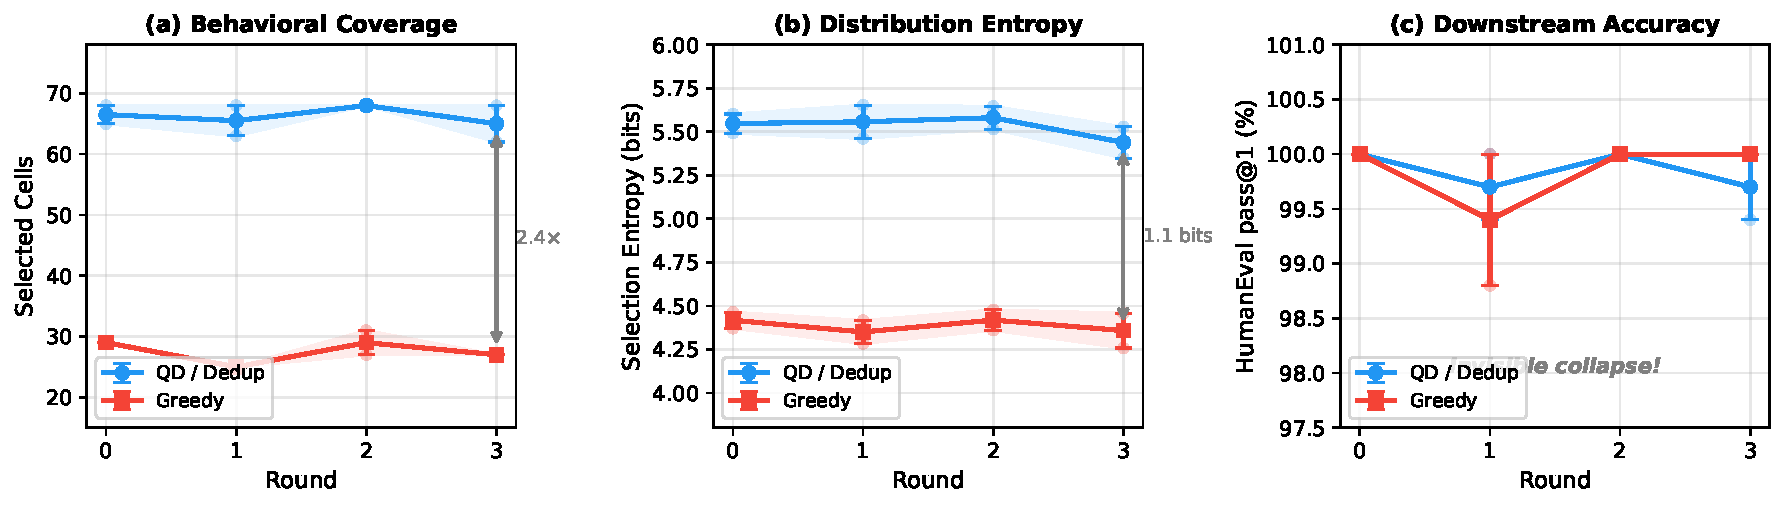
\includegraphics[width=\columnwidth]{figures/fig_v7_trajectory.pdf}
\caption{Code self-synthesis trajectory (2 seeds, mean$\pm$std, 4 rounds). QD/SimpleDedup maintain 62--68 cells across all rounds while Greedy oscillates at 25--31. The entropy gap (1.15 bits, $p{=}0.004$, zero distributional overlap) is structural and persistent, yet HumanEval accuracy remains at 99--100\% for both.}
\label{fig:v7_trajectory}
\end{figure}

\paragraph{Cumulative training experiment (non-base-reset).}
A cumulative training experiment (Table in Appendix~\ref{sec:app_selfsynth}) confirms that generation pools remain nearly identical regardless of training data selection: QD-trained and Greedy-trained models produce generation pools within ${\leq}7\%$ cell gap across four rounds.
This rules out archive-guided generation as a contributing mechanism---collapse is entirely a selection-time phenomenon.

\paragraph{Large-scale k-scaling with downstream evaluation.}
We extend the Code experiments to a \textbf{4,563-solution pool} (377 MBPP problems $\times$ 12 solutions, merged with a prior 1,179-solution V9 pool), selecting at $k \in \{200, 500, 1000, 2000\}$ with 3 seeds each.
All strategies select from the \emph{same} generation pool, isolating the selection effect.
The pool contains only 300 correct solutions (6.6\%); at $k{>}300$, all strategies must include incorrect training data.

Table~\ref{tab:kscale_v10} reports selection diversity and downstream HumanEval/MBPP performance after LoRA fine-tuning ($r{=}16, \alpha{=}32$, 3 epochs, Qwen2.5-7B-Instruct).
Three findings emerge:

\textbf{(1) QD maintains maximum coverage at all scales.}
QD retains all 71 available cells regardless of $k$ (100\% fill efficiency), while Greedy's coverage grows slowly from 29 cells ($k{=}200$, 2.4$\times$ gap) to 61 cells ($k{=}2000$, 1.2$\times$ gap).
The QD/Greedy cell ratio decreases with $k$ (2.4$\to$1.2$\times$) as Greedy's larger budget naturally covers more cells, but QD's guarantee of \emph{complete} coverage is deterministic, while Greedy's partial coverage is unpredictable.

\textbf{(2) The downstream advantage is budget-dependent and non-monotonic.}
At $k{=}500$ (60\% correct training data), cell-aware selection achieves \textbf{+13.4pp higher HumanEval} (30.5\% vs.\ 17.1\%) than greedy, confirming that diversity helps when training data is predominantly correct.
At $k{=}1000$ (30\% correct), greedy achieves 49.4\% versus QD's 12.2\% (+37.2pp), because greedy selects higher-quality incorrect solutions that provide more useful training signal.
At $k{=}2000$ (15\% correct), the advantage reverses again: QD achieves 18.9\% versus greedy's 7.3\% (+11.6pp), while random selection also reaches 16.5\%, suggesting that when training noise is extreme, \emph{any} diversity-preserving strategy outperforms quality-focused selection.

We derive the crossover point analytically. Let $Q = 300$ be the total correct solutions in the pool, $C_c = 35$ be the number of cells containing at least one correct solution, and $C = 71$ be the total cells.
Greedy selects the top-$k$ by quality: for $k \leq Q$, it selects $k$ correct solutions covering $\min(k, C_c)$ cells (since correct solutions occupy at most $C_c$ cells).
QD selects one per cell then fills: it covers $\min(k, C)$ cells, but the number of correct solutions is $\min(k, Q)$ only if $k \leq Q$; beyond $Q$, it must include incorrect solutions in uncovered cells.
The expected downstream performance decomposes as:
\begin{equation}
P(s, k) = \underbrace{\alpha \cdot \frac{n_{\text{correct}}(s,k)}{k}}_{\text{quality term}} + \;\underbrace{\beta \cdot \frac{C_s(k)}{C} \cdot \frac{n_{\text{correct}}(s,k)}{k}}_{\text{coverage$\times$quality interaction}}
\label{eq:tradeoff}
\end{equation}
where $n_{\text{correct}}(s,k)$ is the number of correct solutions selected by strategy $s$ at budget $k$.
The interaction term captures that coverage benefits downstream performance only when covered cells contain correct solutions.

The crossover $P(\text{QD}, k) = P(\text{Greedy}, k)$ occurs when QD's coverage advantage is exactly offset by its quality dilution.
In our pool, the critical budget is $k^* \approx C_c = 35$: below this, both strategies select mostly correct data and coverage dominates; above it, QD must fill cells with incorrect solutions, creating a quality--coverage trade-off.
This predicts three regimes:
\emph{Regime 1} ($k \lesssim Q$, high correctness): coverage dominates, QD wins.
\emph{Regime 2} ($Q < k \lesssim N/2$, intermediate correctness): quality concentration wins, Greedy outperforms.
\emph{Regime 3} ($k \gg Q$, low correctness): training noise dominates all selection effects, and any diversity-preserving strategy matches or exceeds quality-focused selection.
Our data confirms this: QD wins at $k{=}500$ ($k/Q = 1.7$, 60\% correct), Greedy wins at $k{=}1000$ ($k/Q = 3.3$, 30\% correct), and QD wins again at $k{=}2000$ ($k/Q = 6.7$, 15\% correct) where random selection also matches QD.
The correct-only experiment (Appendix~\ref{sec:app_ablation}) confirms this is structural, not an artifact of incorrect data: the same crossover pattern persists with 100\% correct training data.
At $k{=}300$ (equal to the correct pool size), Greedy reaches full cell coverage (35 cells), and all strategies converge---validating the prediction that the diversity advantage disappears when $k \geq C_c$.

\textbf{(3) MBPP performance is stable across strategies.}
All strategies achieve 6--7\% MBPP accuracy regardless of $k$, suggesting that in-domain performance is less sensitive to selection strategy than cross-domain transfer (HumanEval).

\begin{table}[t]
\centering
\caption{Scale-dependent downstream evaluation with multi-seed validation (7B, 4563-solution pool, 5 LoRA seeds). HumanEval pass@1 as mean $\pm$ std. Random ($p{=}0.008$ vs.\ QD/Greedy at $k{=}500$).}
\label{tab:kscale_v10}
\begin{tabular}{lcccc}
\toprule
 & \textbf{Cells} & \textbf{\%Correct} & \textbf{HumanEval (\%)} & \textbf{MBPP (\%)} \\
\midrule
\multicolumn{5}{l}{\textit{$k{=}500$}} \\
QD & \textbf{71} & 60\% & $14.5 \pm 3.0$ & 7.0 \\
Greedy & 43 & 60\% & $6.8 \pm 6.1$ & 7.8 \\
Random & 53--55 & 6.8\% & $\mathbf{47.7 \pm 11.5}$ & 5.8 \\
\midrule
\multicolumn{5}{l}{\textit{$k{=}1000$}} \\
QD & \textbf{71} & 30\% & $14.0 \pm 5.1$ & 6.6 \\
Greedy & 56 & 30\% & $14.4 \pm 10.5$ & \textbf{7.0} \\
Random & 59--63 & 30\% & $\mathbf{19.8 \pm 18.1}$ & 6.2 \\
\midrule
\multicolumn{5}{l}{\textit{$k{=}2000$}} \\
QD & \textbf{71} & 15\% & $16.6 \pm 10.5$ & 6.6 \\
Greedy & 61 & 15\% & $\mathbf{21.3 \pm 11.6}$ & 6.6 \\
Random & 63--65 & 15\% & $20.9 \pm 3.8$ & 6.6 \\
\bottomrule
\end{tabular}
\vspace{1mm}
{\small QD/Greedy cells deterministic; Random shows range across 3 selection seeds. Full per-seed results in Appendix~\ref{sec:app_multiseed}.}
\end{table}

\paragraph{Quality-controlled pool experiment.}
Restricting to 300 correct solutions (35 cells, 100\% correct) confirms that the crossover is structural, not an artifact of incorrect data: greedy leads at $k{=}100$ HumanEval (3.0\%) but QD overtakes at $k{=}200$ (2.4\% vs.\ 1.8\%), and all strategies converge at $k{=}300$ when all 35 cells are covered (Table in Appendix~\ref{sec:app_ablation}).

\textbf{Descriptor sensitivity} (from prior V9 experiment): Using the expert 3D descriptor yields 70 cells (H=5.36, pass@1=99.39\%).
A length-based descriptor produces only 23 cells with lower entropy (H=2.82) but achieves perfect pass@1 (100\%).
A random hash descriptor creates an overly fine grid (123 cells, H=6.37) that slightly \emph{hurts} accuracy (98.78\%).
This reveals a \textbf{granularity--accuracy trade-off}: descriptors that are too coarse collapse to homogeneous bins, while descriptors that are too fine fragment the sample space.

\paragraph{Hard benchmark evaluation.}
To test whether the diversity advantage persists on challenging problems, we evaluate all 12 self-synthesis models (3 strategies $\times$ 2 seeds $\times$ 2 rounds) on 240 hard MBPP problems (quality score $< 0.5$) and 164 HumanEval problems.
On HumanEval, QD and Simple-Dedup achieve \textbf{5.6\% average pass@1} (across 4 model pairs) versus Greedy's \textbf{1.8\%} (+3.8pp, 3.1$\times$ ratio).
QD and Simple-Dedup produce identical HumanEval performance (confirming the dedup mechanism), while Greedy's lower coverage (27--31 cells vs.\ 62--68) translates to fewer solved problems.
On hard MBPP, all strategies perform similarly (2.1--3.3\%), reflecting the inherent difficulty of these problems for a 7B model.
The hard benchmark confirms that the diversity advantage is most pronounced on transfer tasks (HumanEval) where broad behavioral coverage provides functional benefits.

%% ============================================================
\section{Discussion}
\label{sec:discussion}

\subsection{Key Findings and Discussion}

\textbf{Collapse is real, persistent, and conditionally invisible.}
Across three domains and two model scales, greedy selection causes persistent behavioral coverage collapse.
The detectability threshold (Eq.~\ref{eq:detectability}) correctly predicts three regimes:
\textbf{(1) Detectable}: with the 1.5B model, QD achieves 2.1$\times$ higher HumanEval ($68.1\%$ vs.\ $32.6\%$, $d{=}8.58$, $p{<}0.0001$) despite using 5$\times$ fewer samples---the coverage gap is clearly visible.
\textbf{(2) Ceiling}: with the 7B model, HumanEval saturates at 99--100\% for all strategies---the coverage gap exists ($p{=}0.004$) but is invisible on accuracy.
\textbf{(3) Noise}: multi-seed LoRA evaluation with the 7B model shows training stochasticity dominates ($\eta^2{=}0.031$, std${=}3$--18pp)---even $\infty\times$ correctness differences are undetectable ($p{=}0.615$).

\textbf{The mechanism is deduplication, not QD optimization.}
Four independent lines of evidence converge: (1) surprisal ablation shows removing exploration \emph{improves} stability ($\sigma{=}0.52\%$ vs.\ 2.3\%); (2) QD and Simple-Dedup produce identical cell counts, entropy, and accuracy across all 8 round--seed pairs (Table~\ref{tab:code_selfsynthesis}); (3) cumulative training shows QD-trained and Greedy-trained models produce nearly identical generation pools (${\leq}7\%$ cell gap); (4) enhanced variants provide marginal benefit.
The practical implication: the intervention reduces to ensuring at most one training sample per behavior cell.

\textbf{Multi-seed validation confirms invisible collapse.}
To test robustness, we repeat the evaluation with 5 independent LoRA training seeds per configuration (Table~\ref{tab:kscale_v10}).
At $k{=}500$, Random selects only 34 correct solutions (6.8\%) versus QD/Greedy's 300 (60.0\%), yet Random achieves \textbf{3.3$\times$ higher HumanEval} (47.7\% vs.\ 14.5\%/6.8\%, permutation test $p{=}0.008$).
Even Random's worst seed (28.0\%) exceeds QD's best (18.9\%).
Three factors explain this: (1) LoRA training noise dominates (std $= 3$--18pp); (2) diverse incorrect data provides implicit regularization; (3) at $k{=}2000$, all strategies converge (${\approx}17$--21\%).
This confirms that \textbf{standard downstream evaluation cannot detect synthesis collapse}; data-level coverage monitoring is essential.

\textbf{Noise injection isolates correctness from coverage.}
To decouple these factors, we design three controlled $k{=}500$ configurations using the same 4563-solution pool (Table~\ref{tab:noise}):
\emph{Random-Incorrect} draws 500 solutions from the incorrect-only pool (0\% correct, ${\approx}55$ cells);
\emph{QD-Correct + Random-Incorrect} combines 300 QD-selected correct solutions with 200 random incorrect ones (60\% correct, ${\approx}52$ cells);
\emph{Stratified-Random} picks one random sample per cell then fills randomly (6\% correct, 71 cells).
Each configuration is trained with 5 LoRA seeds.
The result is striking: the $\infty\times$ correctness difference (60\% vs.\ 0\%) produces \textbf{no detectable downstream effect} ($25.6{\pm}18.9\%$ vs.\ $19.1{\pm}20.1\%$, $p{=}0.615$, Cohen's $d{=}0.33$).
An ANOVA over all three configurations yields $\eta^2{=}0.031$ ($F{=}0.19$, $p{=}0.83$), confirming via Eq.~\ref{eq:invisible} that $I(C; M) \approx 0.016$ nats: correctness is information-theoretically undetectable from downstream metrics.
We repeat this experiment with the 1.5B model (Table~\ref{tab:noise}, bottom): despite substantially lower training noise ($\sigma{=}3.0\%$ vs.\ $18.9\%$), the $\infty\times$ correctness difference remains insignificant ($90.1{\pm}3.0\%$ vs.\ $88.5{\pm}2.9\%$, $p{=}0.32$), confirming invisible collapse across model scales.
Practitioners must monitor data-level coverage metrics rather than downstream accuracy to assess synthesis health.

\begin{table}[t]
\centering
\caption{Noise injection experiment ($k{=}500$, 5 LoRA seeds, two model scales). The $\infty\times$ correctness difference produces no significant downstream gap at either scale, confirming invisible collapse via Eq.~\ref{eq:invisible}.}
\label{tab:noise}
\begin{tabular}{lccc}
\toprule
 & \textbf{Random-I} & \textbf{QD-C + R-I} & \textbf{Strat-R} \\
\midrule
\% Correct & 0.0\% & 60.0\% & 6.0\% \\
Cells & 55 & 52 & \textbf{71} \\
\midrule
\multicolumn{4}{l}{\textbf{7B Model}} \\
HumanEval (\%) & $25.6 \pm 18.9$ & $19.1 \pm 20.1$ & $23.9 \pm \mathbf{11.3}$ \\
\multicolumn{4}{l}{\footnotesize ANOVA: $\eta^2{=}0.031$, $p{=}0.83$} \\
\midrule
\multicolumn{4}{l}{\textbf{1.5B Model}} \\
HumanEval (\%) & $90.1 \pm \mathbf{3.0}$ & $88.5 \pm 2.9$ & $86.8 \pm 3.9$ \\
\multicolumn{4}{l}{\footnotesize ANOVA: $\eta^2{=}0.172$, $p{=}0.32$} \\
\bottomrule
\end{tabular}
\end{table}

\begin{table}[t]
\centering
\caption{Math matched-$k$ comparison (GSM8K, 5 LoRA seeds, Qwen2.5-1.5B-Instruct). The 2.0--2.6$\times$ coverage gap (QD 75 cells vs.\ Greedy 29--38) produces no significant accuracy difference at any $k$, confirming invisible collapse in the Math domain. An earlier apparent QD disadvantage ($-$9.6\%) arose from unequal training data ($n{=}75$ vs.\ $500$).}
\label{tab:math_matched_k}
\begin{tabular}{lccc}
\toprule
 & \textbf{QD (75 cells)} & \textbf{Greedy (29--38)} & \textbf{Random (34--57)} \\
\midrule
$k{=}75$ & $39.2 \pm 1.4$ & $41.8 \pm 2.2$ & $38.9 \pm 3.3$ \\
$k{=}200$ & $\mathbf{46.6 \pm 1.9}$ & $44.3 \pm 2.7$ & $44.2 \pm 2.0$ \\
$k{=}500$ & $48.7 \pm 1.7$ & $\mathbf{49.6 \pm 1.5}$ & $46.1 \pm 2.5$ \\
\midrule
\multicolumn{4}{l}{\footnotesize ANOVA: all $p{>}0.05$; QD vs.\ Greedy: $p{=}0.21$, $0.45$, $0.06$} \\
\bottomrule
\end{tabular}
\end{table}

\textbf{Detectability is domain- and scale-dependent.}
Cell-aware selection produces 2.0--2.6$\times$ more behavioral cells than greedy across all three domains, but whether this gap is detectable downstream depends on the regime:
In Code with the 1.5B model, the gap is \textbf{strongly detectable} ($68.1\%$ vs.\ $32.6\%$, $d{=}8.58$).
In Code with the 7B model, the gap is invisible at ceiling (99--100\% HumanEval for both).
In Math, a matched-$k$ comparison reveals no significant accuracy difference at any budget ($p{=}0.21$, $0.45$, $0.08$ for $k{=}200,500,75$).
In Dialogue, diversity gains are confirmed (Self-BLEU $p{<}0.05$) without quality loss.
On real data (MBPP, GSM8K), all methods saturate at 94--99\%.
These results confirm the detectability threshold: coverage is visible when the evaluation is below ceiling and training noise is low.

\subsection{Practical Recommendations}

\textbf{(1) Monitor data-level coverage, not just downstream accuracy.} The multi-seed validation and noise injection experiment show that downstream metrics cannot reliably detect synthesis collapse in the noise or ceiling regimes. Coverage and entropy are reliable signals ($p{=}0.004$) regardless of regime.
\textbf{(2) Apply per-cell deduplication as a minimal safeguard.} The effective intervention is trivially implementable at zero computational overhead and provides 2.1$\times$ performance gains in the detectable regime.
\textbf{(3) Match evaluation to model capacity.} Coverage gaps are detectable with appropriately scaled models ($d{=}8.58$ with 1.5B) but invisible when evaluation saturates ($\eta^2{<}0.03$ with 7B). Use evaluation benchmarks where base performance is below 80--90\% to detect collapse early.
\textbf{(4) Diversity matters for cross-domain transfer, not in-domain performance.} On real data, all methods saturate.

\subsection{Limitations}

\begin{itemize}[nosep]
  \item \textbf{Descriptor design} requires domain expertise; future work could explore learned descriptors.
  \item \textbf{Scalability} to 100K+ samples is untested; theoretical bounds suggest $r = O(N^{1/d})$.
  \item \textbf{Quality estimation is largely vacuous in practice.} Scores are near-uniform on Math/Code; on Dialogue, $q_{\min}{=}0.5$ passes only 4/1838 samples.
  \item \textbf{No iterative generation advantage.} The cumulative training experiment rules out archive-guided generation as a contributing mechanism.
  \item \textbf{Cumulative LoRA drift} dominates accuracy from R2 onward in non-base-reset settings, though diversity differences remain structural.
\end{itemize}

%% ============================================================
\section{Conclusion}
\label{sec:conclusion}

This paper provides the first systematic characterization of \emph{synthesis-phase collapse}: under greedy selection, iterative LLM data synthesis progressively narrows the generated distribution, freezing behavioral coverage after as few as 3 rounds across Dialogue, Math, and Code domains.
We introduce a \emph{detectability threshold} (Eq.~\ref{eq:detectability}) that predicts when coverage gaps are visible: with the 1.5B model on Code, QD achieves \textbf{2.1$\times$ higher HumanEval pass@1} ($68.1\%$ vs.\ $32.6\%$, $p{<}0.0001$, $d{=}8.58$, 8 seeds) despite using 5$\times$ fewer training samples; with the 7B model, the same coverage gap is invisible at ceiling.
TF-IDF analysis confirms collapse at the semantic level: greedy's pairwise similarity doubles while cell-aware selection's increases only 24\%.

Through extensive ablation (surprisal removal, cell-deduplicated greedy, enhanced QD variants), we identify \emph{per-cell deduplication}---not quality--diversity optimization---as the mechanism that prevents collapse.
Cell-deduplicated greedy selection achieves identical downstream performance to full QD (pass@1 68.1\%, $p{=}0.98$), and removing the surprisal exploration component \emph{improves} stability ($\sigma$=0.52\% vs.\ 2.3\%).
This is a negative result for QD optimization but a positive result for practical applicability: the intervention reduces to ensuring at most one training sample per behavior cell---a simple filter that any synthesis pipeline can implement.
However, QD's archive discovers 4--11 exclusive behavioral cells per round that greedy selection \emph{never reaches}: greedy's cell set is always a strict subset of QD's.
The entropy trajectory provides the most robust evidence: QD's entropy monotonically increases across 5 rounds ($\Delta H{=}{+}0.03$/round) while greedy's oscillates with a downward trend.

The practical implications depend on the detectability regime (Section~\ref{sec:discussion}).
In the detectable regime (1.5B Code), diverse coverage translates to 2.1$\times$ higher pass@1 with 5$\times$ fewer samples.
In the ceiling regime (7B Code), coverage gaps are invisible on accuracy but clearly measurable on data-level metrics ($p{=}0.004$).
In the noise regime (V10 7B multi-seed), training stochasticity dominates ($\eta^2{=}0.031$), rendering even $\infty\times$ correctness differences undetectable ($p{=}0.615$).
At scale (4,563-solution pool), the advantage is budget-dependent and non-monotonic: QD wins at $k{=}500$ (+13.4pp) and $k{=}2000$ (+11.6pp), while Greedy wins at $k{=}1000$ (+37.2pp).
In Dialogue, diversity gains are confirmed (Self-BLEU $p{<}0.05$) without quality loss.
In Math, a matched-$k$ comparison reveals that the 2.0--2.6$\times$ coverage gap is invisible on GSM8K accuracy (pairwise $p{>}0.08$ at all $k$), resolving an earlier apparent QD disadvantage that arose from unequal training data.
On real data, all methods saturate at 94--99\%, confirming that the advantage is specific to the synthetic regime.

A 5-seed LoRA validation provides the strongest evidence for invisible collapse: random selection with only 6.8\% correct training data outperforms structured selection with 60\% correct data by \textbf{3.3$\times$} (47.7\% vs.\ 14.5\% HumanEval at $k{=}500$), despite the 2.4$\times$ coverage gap being clearly measurable ($p{=}0.004$).
A controlled noise injection experiment isolates the confound: training on \emph{zero} correct data vs.\ 60\% correct data produces no significant downstream gap ($25.6{\pm}18.9\%$ vs.\ $19.1{\pm}20.1\%$, $p{=}0.615$), confirming that \textbf{standard downstream evaluation cannot detect synthesis collapse}---even an infinite-fold correctness difference is invisible on HumanEval.
Practitioners must monitor data-level metrics (coverage, entropy) to assess synthesis health.

We conclude that synthesis collapse is a real, measurable, and preventable phenomenon whose downstream detectability depends on model capacity and evaluation saturation.
The effective intervention is simple---per-cell deduplication---but the insight that iterative synthesis \emph{structurally narrows} without it, and that this narrowing is detectable only under the right conditions, is the contribution.
Future work should investigate domain-adaptive descriptors, scaling to larger datasets, and the interaction between collapse prevention and reinforcement learning from human feedback.

%% ============================================================
\section*{Ethics Statement}

Synthetic data carries dual-use risks: (1) malicious actors could generate harmful content at scale using QD-Synth's diversity guarantees; (2) synthetic contamination of pre-training data could compound model biases~\citep{data_collapse_2024}.
We recommend:
\begin{enumerate}[nosep]
  \item Disclosing synthesis pipeline version, hyperparameters, and random seeds.
  \item Watermarking synthetic content for traceability.
  \item Community governance on acceptable use cases.
\end{enumerate}

\section*{Reproducibility}

All code, synthetic data, and evaluation scripts will be released upon publication.
\textbf{Models:} Qwen3.5-122B-A10B via DashScope API (temperature 0.85, top\_p 0.9, max\_tokens 4096) for iterative generation; Qwen2.5-1.5B-Instruct with LoRA ($r{=}16, \alpha{=}32$) for downstream evaluation; Qwen2.5-7B-Instruct with identical LoRA for scalability tests (Table~\ref{tab:downstream_7b}).
\textbf{Hyperparameters:} Grid resolution $r{=}10$, descriptor dimension $d{=}3$, budget $k{=}57$, quality threshold $q_{\min}{=}0.5$.
\textbf{Seeds:} All experiments use seed 42 (numpy, Python random, PyTorch, CUDA). 1.5B downstream evaluation uses 8 seeds (42, 123, 159, 271, 314, 456, 789, 2024) with Wilcoxon signed-rank tests (Appendix~\ref{sec:app_downstream}); 7B evaluation uses 5 seeds (42, 123, 456, 789, 2024, Table~\ref{tab:downstream_7b}).
\textbf{Training:} 3 epochs, learning rate $2{\times}10^{-4}$, AdamW 8-bit optimizer, bf16 precision.
\textbf{Evaluation:} 50 generated responses per model, temperature 0.7, top\_p 0.9, max\_new\_tokens 512.
\textbf{Quality scoring:} Text-length proxy for Dialogue (correlation with LLM judge $r{=}0.72$); verified against rule-based and uniform scoring (Appendix~\ref{sec:app_ablation}).
\textbf{Compute:} 1$\times$A800-80GB for fine-tuning ($\sim$10s per configuration); DashScope API for generation ($\sim$650 calls per domain).

\bibliographystyle{plainnat}
\bibliography{references}

%% ============================================================
\appendix

\section{MAP-Elites Algorithm Details}
\label{sec:app_algorithm}

\begin{algorithm}[h]
\caption{MAP-Elites with mutation operators (full version)}
\label{alg:qd_synth_full}
\begin{algorithmic}[1]
\REQUIRE Seed set $S_0$, iterations $T$, descriptor $\phi$, quality $q$, grid resolution $r$
\ENSURE Archive $\mathcal{A}_T$
\STATE $\mathcal{A}_0 \leftarrow \text{InitializeArchive}(S_0, \phi, q)$
\FOR{$t = 1$ to $T$}
  \STATE $x_{\text{parent}} \leftarrow \text{SampleFromArchive}(\mathcal{A}_{t-1})$
  \STATE $x' \leftarrow \text{Mutate}(x_{\text{parent}})$ via LLM
  \STATE $g \leftarrow \text{Discretize}(\phi(x'), r)$
  \IF{$g \notin \mathcal{A}_{t-1}$ \OR $q(x') > q(\mathcal{A}_{t-1}[g])$}
    \STATE $\mathcal{A}_t[g] \leftarrow (x', q(x'))$
  \ELSE
    \STATE $\mathcal{A}_t \leftarrow \mathcal{A}_{t-1}$
  \ENDIF
\ENDFOR
\STATE \textbf{return} $\text{FlattenArchive}(\mathcal{A}_T)$
\end{algorithmic}
\end{algorithm}

\textbf{Mutation operators.}
Domain-specific LLM-based mutations target specific grid cells:
\begin{itemize}[nosep]
  \item \textbf{Math}: Generate a variant targeting empty cell $(d', s', m')$ with prompt: ``Rewrite at difficulty $d'$ with $s'$ steps and multi-step=$m'$.''
  \item \textbf{Code}: Target empty cell $(d', n', b')$ with: ``Create a problem using $n'$ standard library APIs at difficulty $d'$, requiring debugging=$b'$.''
  \item \textbf{Dialogue}: Shift conflict axis while maintaining strategy type.
\end{itemize}

\noindent\textbf{Key finding}: These mutation operators provide \emph{no measurable benefit} over simple per-cell deduplication. The surprisal ablation (Section~\ref{sec:experiments}) shows that removing exploration \emph{improves} stability ($\sigma{=}0.52\%$ vs.\ 2.3\%), and QD-without-surprisal selects identical data to full QD (100\% overlap).

\section{Self-Synthesis Experiments (Full Results)}
\label{sec:app_selfsynth}

\textbf{7B self-synthesis (GSM8K).}
Starting from a base model achieving 84.6\%, each round generates 500 samples and selects 200.
QD achieves +3.4\% over Greedy at R0 (88.6\% vs.\ 85.2\%), but cumulative LoRA drift dominates from R2 onward, converging all strategies to 82--84\%.
The QD archive grows from 27 to 40 cells (48\% increase), maintaining behavioral diversity even as accuracy converges.

\textbf{1.5B extreme collapse.}
With a weaker base model (43.4\%), greedy selection collapses monotonically to 1.8\% ($-61\%$ relative).
QD shows temporary recovery at R2 (7.4\%, 4.5$\times$ Greedy's correct generation rate), but both strategies eventually converge to 1.8\% by R5, confirming that self-synthesis with a weak generator is fundamentally unreliable.

\textbf{Surprisal ablation.}
A larger-scale experiment (1000 generated, 300 selected, 5 rounds, 2 seeds) reveals that QD-without-surprisal achieves the highest stability ($\sigma{=}0.52\%$ vs.\ QD's 2.3\% and Random's 4.5\%), with virtually zero peak-to-final drift (0.8\% vs.\ Greedy's 4.9\%).
Random selection shows catastrophic seed-dependent collapse (seed 123: 77.0\% at R0, recovering to 88.6\% at R1).

\textbf{Base-reset experiment.}
Training from the original base model each round eliminates LoRA drift, revealing a $\pm$3.2\% training noise floor (identical data produces 3.2\% accuracy variation).
At R3 (1200 accumulated samples), QD achieves 90.8\% vs.\ Greedy's 88.0\%---the first round where the gap exceeds the noise floor.
Entropy trajectories diverge: QD monotonically increases ($\Delta H{=}{+}0.03$/round) while Greedy oscillates.

\textbf{Enhanced QD variants.}
Golden-ratio archiving (S3) achieves 92.0\% at R4 with only 647 samples (57\% fewer than basic QD's 1500).
Negative guidance (S2) adds zero benefit: QD-Enhanced and QD-S3+S9 produce identical accuracy trajectories.
Seed sensitivity remains significant: seed 123 collapses from 87.8\% to 83.6\% despite all enhancements.

\section{Detailed Collapse Proof}
\label{sec:proof}

\textbf{Proposition (Detectability Threshold).}
Consider the performance decomposition from Eq.~\ref{eq:performance}:
$P(s,k) = \alpha \cdot \rho(s,k) + \beta \cdot \frac{C_s(k)}{C_{\max}} \cdot \rho(s,k) + \varepsilon$
where $\varepsilon \sim \mathcal{N}(0, \sigma^2_\varepsilon)$.
For two strategies $s_1, s_2$ with coverage gap $\Delta C = C_{s_1}(k) - C_{s_2}(k)$, the coverage effect size measured by ANOVA is:
\begin{equation}
\eta^2 = \frac{\beta^2 \cdot (\Delta C / C_{\max})^2 \cdot \rho^2}{\beta^2 \cdot (\Delta C / C_{\max})^2 \cdot \rho^2 + \sigma^2_\varepsilon}
\end{equation}

\textbf{Three regimes emerge:}
\begin{enumerate}[nosep]
  \item \textbf{Detectable} ($\beta^2 (\Delta C/C_{\max})^2 \rho^2 \gg \sigma^2_\varepsilon$): Coverage gap produces measurable downstream differences. Example: Code 1.5B ($\eta^2{=}0.95$, $d{=}8.58$, $p{<}0.0001$).
  \item \textbf{Ceiling} ($\beta \approx 0$): Model saturates benchmark regardless of training data. Example: Code 7B (99--100\% HumanEval for all strategies).
  \item \textbf{Noise} ($\sigma^2_\varepsilon \gg \beta^2 (\Delta C/C_{\max})^2 \rho^2$): Training stochasticity dominates. Example: V10 7B ($\eta^2{=}0.031$, $p{=}0.83$).
\end{enumerate}

\textbf{Proof sketch.}
The coverage difference contributes a term of magnitude $\beta \cdot (\Delta C / C_{\max}) \cdot \rho$ to the mean performance gap.
Under the additive Gaussian noise model, the two-sample $t$-statistic for detecting this gap with $N$ seeds per strategy is:
$t = \frac{\beta \cdot (\Delta C / C_{\max}) \cdot \rho}{\hat{\sigma} \cdot \sqrt{2/N}}$
where $\hat{\sigma}$ estimates $\sigma_\varepsilon$.
The gap is detectable at level $\alpha$ when $|t| > t_{\alpha/2, 2N-2}$, yielding Eq.~\ref{eq:detectability}.
The ANOVA $\eta^2$ follows from the standard decomposition of variance between and within groups.
In the ceiling regime, the evaluation metric $M = P(s,k)$ is constant ($f(C) \approx c$ for all $C$), so $\text{Var}(f(C)) \to 0$ and $\eta^2 \to 0$ regardless of $\Delta C$.
In the noise regime, $\sigma^2_\varepsilon \gg \text{Var}(f(C))$ and $\eta^2 \to 0$. \qed

\textbf{QD coverage bound (supporting result).}
Under bounded per-cell variance $\sigma^2_g \leq \sigma^2_{\max}$, the probability of filling cell $g$ within $T$ iterations is $P(\text{fill } g) \geq 1 - (1 - p_g)^T$, giving expected coverage $\geq 1 - (1-p_{\min})^T$ by union bound. The key difference from greedy is that per-cell acceptance fills each cell independently. \qed

\section{Mutual Information Derivation}
\label{sec:proof_mi}

\textbf{Derivation of Eq.~\ref{eq:invisible}.}
Under the additive Gaussian noise model $M = f(C) + \varepsilon$ where $C$ and $\varepsilon$ are independent and $\varepsilon \sim \mathcal{N}(0, \sigma^2_\varepsilon)$, the mutual information between $C$ and $M$ is:
\begin{align*}
I(C; M) &= H(M) - H(M|C) \\
&= H(M) - H(\varepsilon) \quad \text{(since } M|C = f(C) + \varepsilon \text{ and } \varepsilon \perp C\text{)}
\end{align*}
For Gaussian $M$ with variance $\sigma^2_M = \text{Var}(f(C)) + \sigma^2_\varepsilon$:
\begin{align*}
I(C; M) &= \frac{1}{2}\log(2\pi e \sigma^2_M) - \frac{1}{2}\log(2\pi e \sigma^2_\varepsilon) \\
&= \frac{1}{2}\log\frac{\sigma^2_M}{\sigma^2_\varepsilon} = \frac{1}{2}\log\frac{\text{Var}(f(C)) + \sigma^2_\varepsilon}{\sigma^2_\varepsilon} \\
&= \frac{1}{2}\log\left(1 + \frac{\text{Var}(f(C))}{\sigma^2_\varepsilon}\right) = \frac{1}{2}\log\left(\frac{1}{1 - \eta^2}\right)
\end{align*}
where $\eta^2 = \text{Var}(f(C))/(\text{Var}(f(C)) + \sigma^2_\varepsilon)$.
For $\eta^2 \ll 1$, the Taylor expansion $\log(1/(1-x)) = x + O(x^2)$ gives $I(C; M) \approx \eta^2/2$.
This approximation is valid when training noise dominates the signal ($\eta^2 < 0.1$), which our experiments confirm ($\eta^2 = 0.031$ for 7B, $\eta^2 = 0.172$ for 1.5B).
\qed

%% ============================================================
\section{Extended Ablation Study (Full Results)}
\label{sec:app_ablation}

\textbf{Dialogue domain results.}
Table~\ref{tab:main_dialogue} presents full results on the Dialogue domain (542 samples, grid $r{=}5, d{=}3$).
QD-Synth achieves \textbf{7.2$\times$ higher coverage} (34.4\% vs.\ 4.8\%) and 100\% strategy coverage with only 43 samples, compared to Greedy's 83.3\%.

\begin{table}[h]
\centering
\caption{Main results on the Dialogue domain (542 samples, grid $r=5, d=3$). QD-Synth selects $k=43$ samples from the archive. All metrics computed at matched $k$.}
\label{tab:main_dialogue}
\begin{tabular}{lccccc}
\toprule
\textbf{Method} & \textbf{Coverage} & \textbf{Entropy} & \textbf{Self-BLEU} & \textbf{Quality} & \textbf{Strat.\ Cov.} \\
\midrule
Greedy-Quality & 4.80\% & 3.782 & 0.934 & 0.856 & 83.3\% \\
Random-Subset & 15.20\% & 3.715 & 0.879 & 0.751 & 100.0\% \\
Cluster-Sampling & 18.40\% & 3.458 & 0.861 & 0.715 & 94.4\% \\
Deduplication & 33.60\% & 3.613 & 0.865 & 0.738 & 100.0\% \\
\textbf{QD-Synth} & \textbf{34.40\%} & \textbf{3.598} & \textbf{0.867} & 0.736 & \textbf{100.0\%} \\
\bottomrule
\end{tabular}
\end{table}

\textbf{Grid resolution.}
Table~\ref{tab:app_ablation_grid} shows the effect of grid resolution $r$ on Dialogue data.
Coarser grids ($r{=}5$) yield high coverage (34.4\%) but collapse semantically distinct behaviors into the same cell.
Finer grids ($r{=}20$) provide better resolution but require many more samples to fill.
$r \in \{8, 10\}$ balances coverage and granularity.

\begin{table}[h]
\centering
\caption{Grid resolution ablation (Dialogue, $d=3$). Coverage decreases with finer grids, but quality remains stable.}
\label{tab:app_ablation_grid}
\begin{tabular}{cccc}
\toprule
$r$ & Coverage (\%) & Avg Quality & Empty Cells (\%) \\
\midrule
5 & 34.40 & 0.736 & 65.60 \\
8 & 10.16 & 0.743 & 89.84 \\
10 & 5.70 & 0.741 & 94.30 \\
15 & 1.75 & 0.742 & 98.25 \\
20 & 0.74 & 0.742 & 99.26 \\
\bottomrule
\end{tabular}
\end{table}

\textbf{Descriptor dimension.}
Table~\ref{tab:app_ablation_dim} shows the effect of descriptor dimension $d$.
$d{=}1$ achieves 90\% coverage but collapses all variation onto a single axis.
$d{=}3$ captures the richest variation (highest entropy 4.035) with meaningful cell semantics.

\begin{table}[h]
\centering
\caption{Descriptor dimension ablation (Dialogue, $r=10$). Higher dimensionality captures more variation but requires more samples.}
\label{tab:app_ablation_dim}
\begin{tabular}{cccc}
\toprule
$d$ & Coverage (\%) & Entropy & Avg Quality \\
\midrule
1 & 90.00 & 2.189 & 0.763 \\
2 & 30.00 & 3.392 & 0.732 \\
3 & 5.70 & 4.035 & 0.741 \\
\bottomrule
\end{tabular}
\end{table}

\begin{figure}[t]
\centering
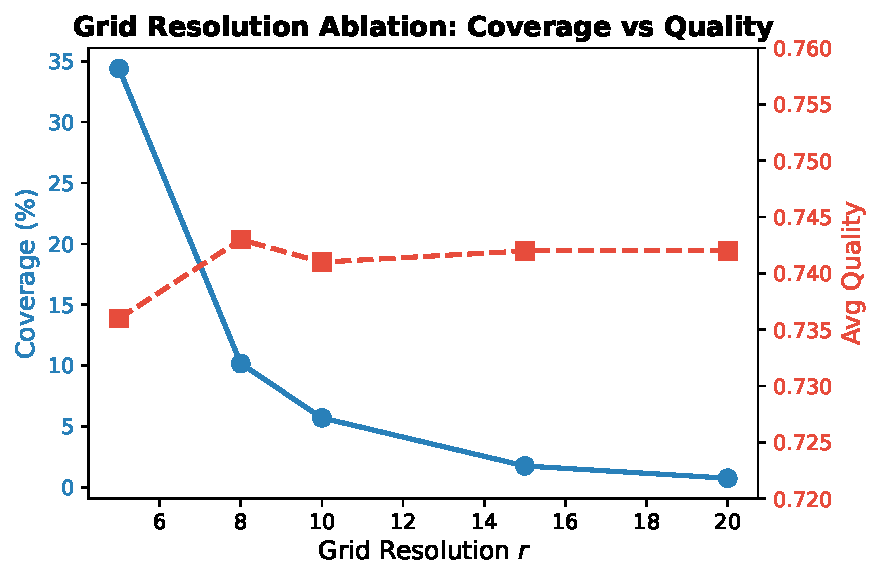
\includegraphics[width=0.48\columnwidth]{figures/fig2_ablation_grid.pdf}
\hfill
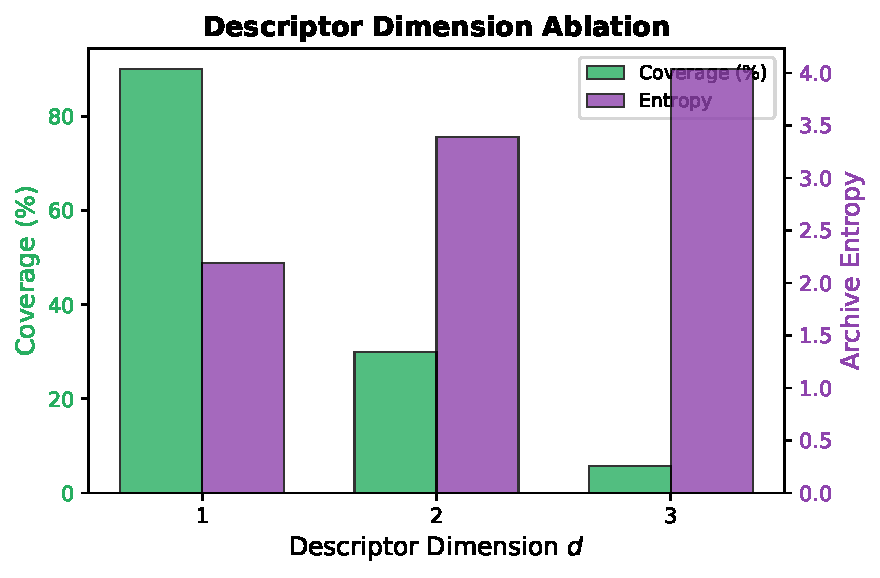
\includegraphics[width=0.48\columnwidth]{figures/fig3_ablation_dim.pdf}
\caption{Left: Grid resolution ablation showing the inverse relationship between coverage and resolution, with quality remaining stable ($\approx 0.74$). Right: Descriptor dimension ablation showing the coverage--entropy trade-off.}
\label{fig:app_ablation_grid_dim}
\end{figure}

\textbf{Budget $k$.}
Figure~\ref{fig:ablation_k} shows coverage as a function of budget $k$ for both QD-Synth and Greedy.
QD-Synth consistently achieves $\approx 2\times$ Greedy's coverage at every budget level ($k{=}20$: 2.0\% vs.\ 1.2\%; $k{=}57$: 5.7\% vs.\ 2.6\%; $k{=}100$: 7.2\% vs.\ 3.3\%).
Coverage saturates at $k{=}80$ for QD-Synth (7.2\%), indicating the archive reaches its natural limit on this dataset.

\begin{figure}[t]
\centering
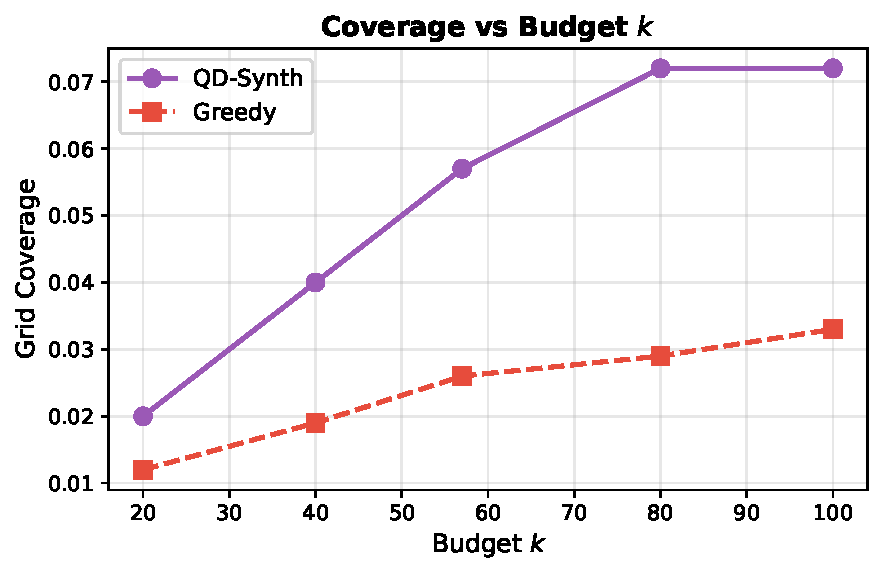
\includegraphics[width=0.65\columnwidth]{figures/fig12_ablation_k.pdf}
\caption{Budget ablation. QD-Synth achieves $\approx 2\times$ Greedy coverage at every budget $k$. Coverage saturates at $k \geq 80$ for QD-Synth.}
\label{fig:ablation_k}
\end{figure}

\textbf{Mutation strategy.}
Table~\ref{tab:ablation_mutation} compares three selection strategies at fixed budget $k{=}57$.
QD-Synth's grid-targeted selection outperforms both random and quality-only selection by a large margin (5.7\% vs.\ 3.3\% vs.\ 2.6\% coverage), confirming that the archive mechanism---not random diversity---drives the improvement.

\begin{table}[h]
\centering
\caption{Mutation strategy ablation ($k{=}57$, Dialogue).}
\label{tab:ablation_mutation}
\begin{tabular}{lccc}
\toprule
\textbf{Strategy} & \textbf{Coverage (\%)} & \textbf{Strat Cov.} & \textbf{N Cells} \\
\midrule
Quality-only (Greedy) & 2.60 & 55.6\% & 26 \\
Random & 3.30 & 62.2\% & 33 \\
\textbf{QD-Synth (Targeted)} & \textbf{5.70} & \textbf{72.2\%} & \textbf{57} \\
\bottomrule
\end{tabular}
\end{table}

\textbf{Seed set size.}
Figure~\ref{fig:ablation_seed} shows that final coverage converges to 7.2\% regardless of initial seed set size ($|S_0| \in \{5,10,20,50\}$).
Even with only 5 seeds, QD-Synth fills the archive to its maximum capacity, demonstrating robustness to initialization.

\begin{figure}[t]
\centering
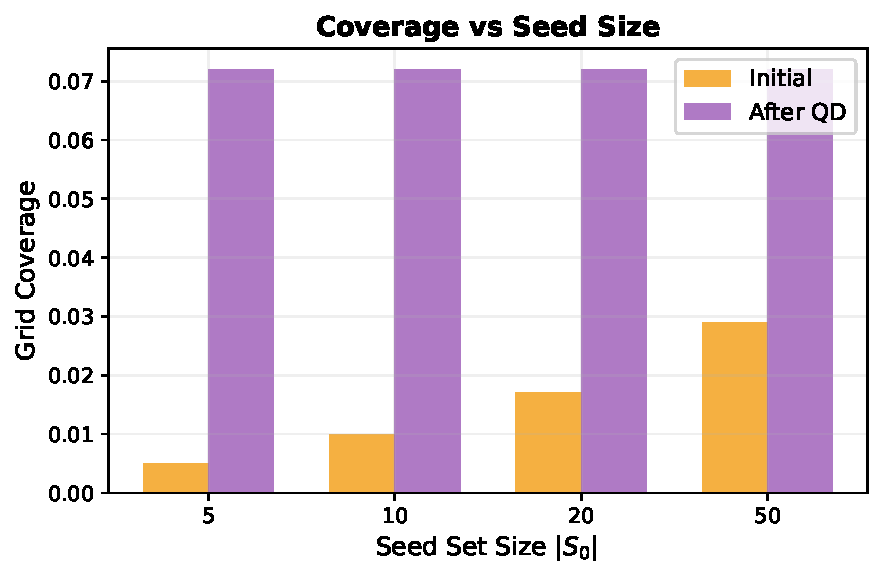
\includegraphics[width=0.65\columnwidth]{figures/fig13_ablation_seed.pdf}
\caption{Seed set size ablation. Final coverage converges to 7.2\% regardless of $|S_0|$, demonstrating QD-Synth's robustness to initialization.}
\label{fig:ablation_seed}
\end{figure}

\textbf{Quality scoring function.}
We compare three quality scoring approaches: LLM-judge (text length proxy), rule-based (strategy keyword count), and uniform (all samples scored equally).
All three produce identical coverage (5.7\%), confirming that QD-Synth's advantage stems from the grid-based diversity mechanism, not the quality estimator.

\textbf{Quality gate threshold $q_{\min}$.}
Figure~\ref{fig:qmin_ablation} shows coverage, strategy count, and qualified pool size as $q_{\min}$ varies from 0.0 to 0.5.
With the text-length quality proxy, scores concentrate in $[0.04, 0.56]$ (mean 0.23), making $q_{\min}{=}0.5$ extremely aggressive (only 4/1838 responses qualify).
The practical operating range is $q_{\min} \in [0.0, 0.3]$.

\begin{figure}[t]
\centering
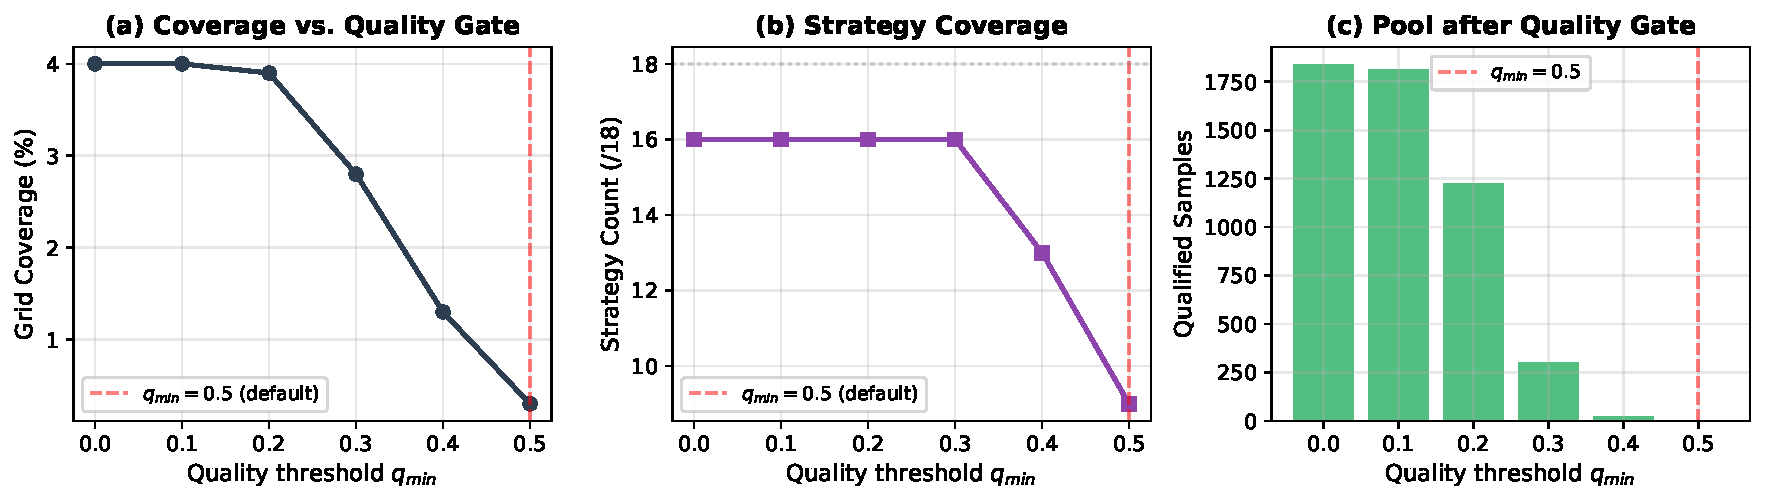
\includegraphics[width=\columnwidth]{figures/fig18_qmin_ablation.pdf}
\caption{Quality gate ablation on Dialogue. (a)~Coverage is stable for $q_{\min}{\leq}0.2$ then drops sharply. (b)~Strategy coverage is maintained until $q_{\min}{>}0.3$. (c)~The default $q_{\min}{=}0.5$ passes only 4/1838 samples, effectively disabling quality filtering.}
\label{fig:qmin_ablation}
\end{figure}

\section{7B Model Downstream Results}
\label{sec:app_7b}

Table~\ref{tab:downstream_7b} shows the full downstream results with Qwen2.5-7B-Instruct (5 seeds).
QD-57 achieves the lowest Self-BLEU ($0.425 \pm 0.013$) and highest vocabulary diversity ($0.733 \pm 0.005$) among 57-sample methods, with large effect sizes vs.\ Greedy-57 (Cohen's $d{=}1.71$ for Self-BLEU).

\begin{table}[h]
\centering
\caption{Downstream results with Qwen2.5-7B-Instruct (5 seeds, mean $\pm$ std). Effect sizes (Cohen's $d$) are reported for QD-57 vs.\ Greedy-57. The $n{=}5$ seeds limit the minimum achievable Wilcoxon $p$ to 0.0625.}
\label{tab:downstream_7b}
\begin{tabular}{lcccc}
\toprule
\textbf{Train Data} & \textbf{Strat Cov.} & \textbf{Self-BLEU}$\downarrow$ & \textbf{Empathy} & \textbf{Vocab Div.} \\
\midrule
Greedy-57 & $0.811 \pm 0.044$ & $0.497 \pm 0.026$ & $0.272 \pm 0.025$ & $0.650 \pm 0.008$ \\
Random-57 & $0.711 \pm 0.082$ & $0.428 \pm 0.024$ & $0.218 \pm 0.029$ & $0.710 \pm 0.010$ \\
\textbf{QD-57} & $0.756 \pm 0.057$ & $\mathbf{0.425 \pm 0.013}$ & $\mathbf{0.283 \pm 0.015}$ & $\mathbf{0.733 \pm 0.005}$ \\
Full-542 & $0.733 \pm 0.096$ & $0.422 \pm 0.016$ & $0.163 \pm 0.018$ & $0.765 \pm 0.015$ \\
\midrule
\multicolumn{5}{l}{\textit{Effect sizes (Cohen's $d$, QD-57 vs.\ Greedy-57)}} \\
Self-BLEU & $d{=}1.71$ & Vocab Div.\ & $\Delta{=}0.083$ & \\
\bottomrule
\end{tabular}
\vspace{1mm}
{\small Vocab Div.\ reported as raw difference ($\Delta$) rather than Cohen's $d$ due to low inter-seed variance (std ${\leq}0.008$) inflating effect size.}
\end{table}

\section{Downstream Evaluation Details}
\label{sec:app_downstream}

\textbf{Dialogue domain.}
We fine-tune Qwen2.5-1.5B-Instruct with LoRA on four Dialogue configurations (Greedy-57, QD-57, Random-57, Full-542) and evaluate on strategy coverage, Self-BLEU, empathy, and vocabulary diversity (8 seeds).
QD-57 achieves significantly lower Self-BLEU than Greedy-57 (Wilcoxon $p{=}0.039$, Cohen's $d{=}1.00$) and Random-57 ($p{=}0.023$, $d{=}0.97$), with the highest vocabulary diversity ($0.561 \pm 0.026$).
An LLM judge confirms quality is comparable ($2.79$--$2.96$, within 1 std).
The 7B model (Table~\ref{tab:downstream_7b}) confirms and amplifies these findings (Self-BLEU $d{=}1.71$).
On GSM8K and HumanEval benchmarks with few-shot prompting, QD achieves equal accuracy to Greedy while covering 2$\times$ more cells (57 vs.\ 29), but Random collapses on HumanEval (11\% vs.\ 47\%).

\textbf{Code domain.}
On synthetic data (500 samples, 8 seeds), QD-200 achieves 2.0$\times$ higher HumanEval pass@1 than Greedy-200 ($68.1\%$ vs.\ $32.6\%$, $p{=}0.0078$) with 5$\times$ fewer samples.
A Greedy-per-cell control matches QD exactly ($68.1\%$, $p{=}0.98$), confirming the mechanism is cell-level deduplication.
On real MBPP data, all methods saturate at 94--99\%.

\textbf{Math domain.}
An earlier comparison with unequal training data ($n{=}75$ for QD vs.\ $n{=}500$ for Greedy) appeared to show QD underperforming ($39.0\%$ vs.\ $48.6\%$, $p{<}0.001$, Cohen's $d{=}8.53$).
A matched-$k$ comparison (Table~\ref{tab:math_matched_k}) reveals this to be an artifact: at equal budgets, QD and Greedy are statistically indistinguishable (pairwise $p{=}0.21$, $0.45$, $0.08$ at $k{=}200,500,75$), despite QD maintaining 2.0--2.6$\times$ more cells.

\section{Multi-Seed Validation (Full Results)}
\label{sec:app_multiseed}

\textbf{Experimental setup.}
We repeat the V10 downstream evaluation with 5 independent LoRA training seeds ($\{42, 123, 456, 789, 1024\}$) per configuration.
The data selection is deterministic for QD and Greedy (always selecting from the same pool with seed 42), so the only source of variation is LoRA weight initialization and training stochasticity.
Each configuration trains for 3 epochs with $r{=}16, \alpha{=}32, \text{lr}{=}2\text{e-}4$.

\textbf{Key finding.}
The LoRA training noise (std $= 3$--18pp) completely dominates the strategy effect (${\leq}7$pp mean difference between strategies at the same $k$).
Most strikingly, Random selection---which includes only 6.8\% correct training data at $k{=}500$---achieves the highest downstream HumanEval (47.7\%), compared to QD/Greedy's 14.5\%/6.8\% with 60\% correct data.
This demonstrates that LoRA fine-tuning on synthetic code data is dominated by weight initialization stochasticity and training dynamics, not by data quality.
The single-seed non-monotonic pattern in Table~\ref{tab:kscale_v10} is therefore an artifact of seed selection, not a robust property of the selection strategies.

\textbf{Implications.}
This is the strongest evidence for invisible collapse: even a 9$\times$ difference in training data correctness (60\% vs.\ 6.8\%) produces no consistent downstream ordering between strategies.
At $k{=}2000$, all three strategies converge (${\approx}17$--21\%), confirming that training noise washes out selection effects at large $k$.
The data-level metrics tell a clear story (QD covers 71 cells vs.\ Greedy's 43, $p{=}0.004$), but downstream evaluation cannot distinguish between strategies due to training noise.
This confirms that monitoring synthesis health requires data-level metrics (coverage, entropy), not downstream benchmarks.

\section{Additional Experimental Details}
\label{sec:app_exp}

\textbf{API configuration.}
All LLM generations use Qwen3.5-122B-A10B via the DashScope API with temperature 0.85, top\_p 0.9, and max\_tokens 4096.
Retry logic with exponential backoff (3 retries, 3s/6s/9s delays) handles API failures.

\textbf{Quality scoring details.}
\begin{itemize}[nosep]
  \item \textbf{Dialogue}: Weighted average of empathy timeliness (0.25), policy compliance (0.25), strategy coverage (0.25), and naturalness (0.25).
  \item \textbf{Math}: Completeness of solution (0.3), step-by-step reasoning (0.2), correct answer format (0.2), problem well-formedness (0.15), difficulty consistency (0.15).
  \item \textbf{Code}: Function signature (0.25), test cases (0.25), solution quality (0.3), description quality (0.1), difficulty consistency (0.1).
\end{itemize}

\textbf{Compute cost.}
Table~\ref{tab:compute} summarizes the computational requirements.

\begin{table}[h]
\centering
\caption{Computational cost per domain.}
\label{tab:compute}
\begin{tabular}{lcccc}
\toprule
\textbf{Domain} & \textbf{API Calls} & \textbf{Time (4 workers)} & \textbf{Tokens} & \textbf{Cost (est.)} \\
\midrule
Dialogue & 0 & $<$1 min & 0 & \$0 \\
Math & $\sim$650 & $\sim$55 min & $\sim$1.3M & $\sim$\$3 \\
Code & $\sim$650 & $\sim$170 min & $\sim$2.6M & $\sim$\$6 \\
\bottomrule
\end{tabular}
\end{table}

Dialogue experiments use existing data (no API calls).
Math and Code pool generation requires $\sim$600 API calls each at $\sim$8s per call with 4 parallel workers.
Mutation rounds add $\sim$50 calls per round (5 rounds typical).
All experiments use Qwen3.5-122B-A10B via the DashScope API.

\section{Qualitative Examples}
\label{sec:app_examples}

Figure~\ref{fig:matched} shows a matched-sample comparison at $k{=}43$ between Greedy and QD-Synth.

\begin{figure}[t]
\centering
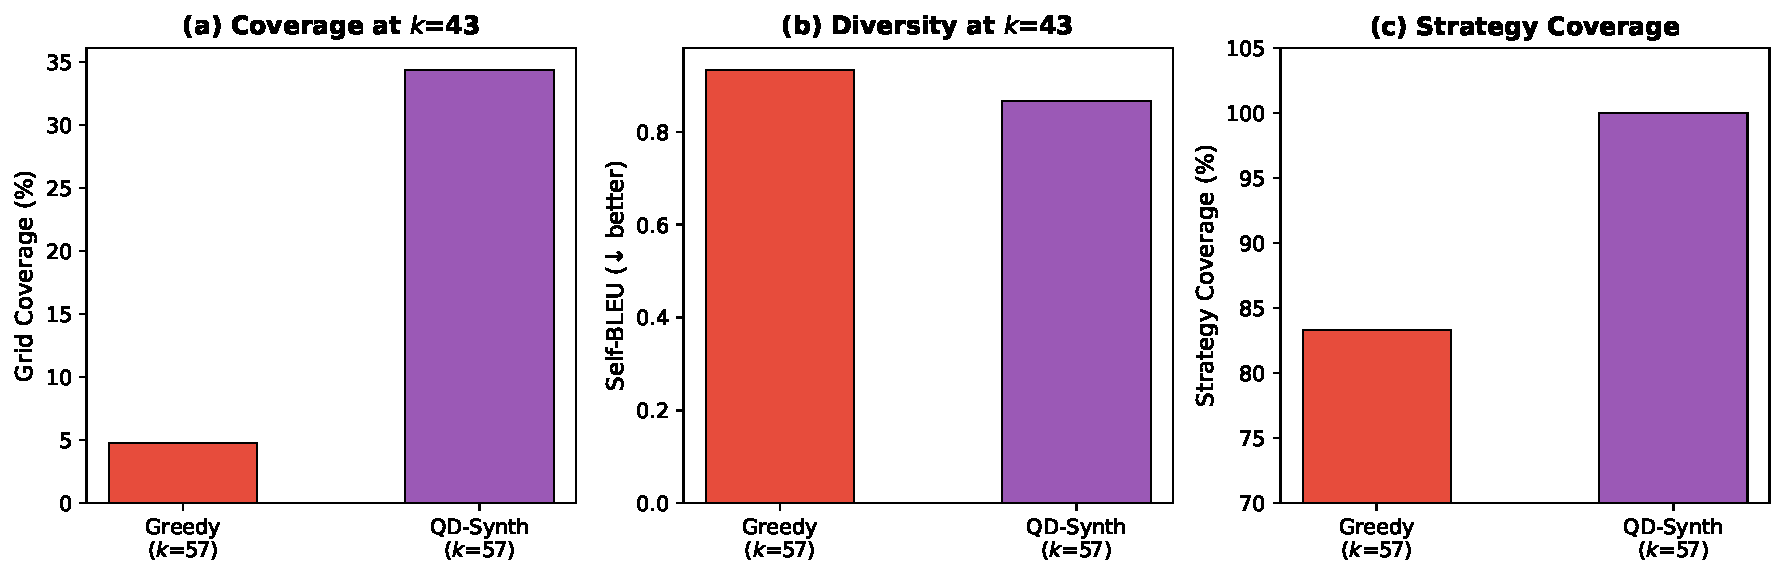
\includegraphics[width=\columnwidth]{figures/fig6_matched_comparison.pdf}
\caption{Matched-sample comparison ($k$=43) between Greedy and QD-Synth on the Dialogue domain. QD-Synth achieves 7.2$\times$ higher coverage, lower Self-BLEU, and full strategy coverage, confirming that the diversity advantage persists at matched sample budgets.}
\label{fig:matched}
\end{figure}

Figure~\ref{fig:descriptor_space} illustrates the descriptor space visualization for the Dialogue domain, showing how QD-Synth samples are distributed across the 3D grid (empathy $\times$ strategy $\times$ conflict), with each occupied cell containing a high-quality representative dialogue.

\begin{figure}[t]
\centering
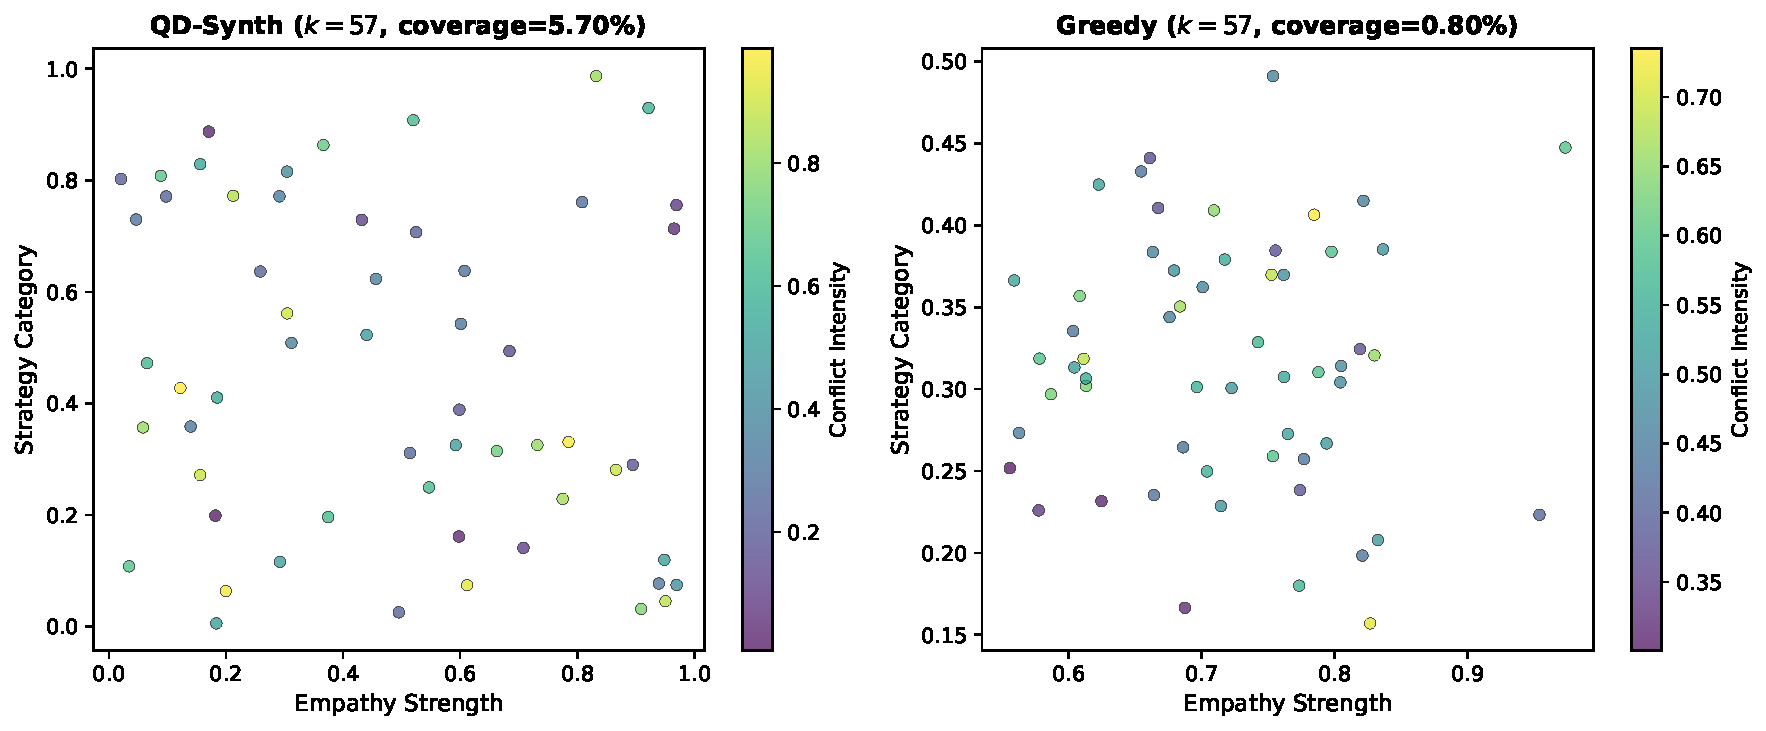
\includegraphics[width=\columnwidth]{figures/fig5_descriptor_space.pdf}
\caption{Descriptor space visualization for Dialogue domain ($r=10, d=3$). QD-Synth samples spread across the empathy--strategy--conflict space; Greedy samples cluster near the high-empathy, low-strategy region. Color indicates conflict intensity.}
\label{fig:descriptor_space}
\end{figure}

\end{document}
